\documentclass[a4paper, 12pt]{report}

\usepackage[dvipsnames]{xcolor}

%%%%%%%%%%%%%%%%
% Set Variables %
%%%%%%%%%%%%%%%%

\def\useItalian{0}  % 1 = Italian, 0 = English

\def\courseName{Cryptography}

\def\coursePrerequisites{Algebra and Computational Complexity}

\def\book{"Introduction to Modern Cryptography", J. Katz, Y. Lindell}

\def\authorName{Simone Bianco}
\def\email{bianco.simone@outlook.it}
\def\github{https://github.com/Exyss/university-notes}
\def\linkedin{https://www.linkedin.com/in/simone-bianco}

% \def\authorName{Alessio Bandiera}
% \def\email{alessio.bandiera02@gmail.com}
% \def\github{https://github.com/aflaag-notes}
% \def\linkedin{https://www.linkedin.com/in/alessio-bandiera-a53767223}

%%%%%%%%%%%%
% Packages %
%%%%%%%%%%%%

\usepackage{../../packages/Nyx/nyx-packages}
\usepackage{../../packages/Nyx/nyx-styles}
\usepackage{../../packages/Nyx/nyx-frames}
\usepackage{../../packages/Nyx/nyx-macros}
\usepackage{../../packages/Nyx/nyx-title}
\usepackage{../../packages/Nyx/nyx-intro}

%%%%%%%%%%%%%%
% Title-page %
%%%%%%%%%%%%%%

\logo{../../packages/Nyx/logo.png}

\if\useItalian1
    \institute{\curlyquotes{\hspace{0.25mm}Sapienza} Università di Roma}
    \faculty{Ingegneria dell'Informazione,\\Informatica e Statistica}
    \department{Dipartimento di Informatica}
    \ifdefined\book
        \subtitle{Appunti integrati con il libro \book}
    \fi
    \author{\textit{Autore}\\\authorName}
\else
    \institute{\curlyquotes{\hspace{0.25mm}Sapienza} University of Rome}
    \faculty{Faculty of Information Engineering,\\Informatics and Statistics}
    \department{Department of Computer Science}
    \ifdefined\book
        \subtitle{Lecture notes integrated with the book \book}
    \fi
    \author{\textit{Author}\\\authorName}
\fi


\title{\courseName}
\date{\today}

% \supervisor{Linus \textsc{Torvalds}}
% \context{Well, I was bored\ldots}

%%%%%%%%%%%%
% Document %
%%%%%%%%%%%%

\begin{document}
    \maketitle

    % The following style changes are valid only inside this scope 
    {
        \hypersetup{allcolors=black}
        \fancypagestyle{plain}{%
        \fancyhead{}        % clear all header fields
        \fancyfoot{}        % clear all header fields
        \fancyfoot[C]{\thepage}
        \renewcommand{\headrulewidth}{0pt}
        \renewcommand{\footrulewidth}{0pt}}

        \romantableofcontents
    }

    \introduction

    %%%%%%%%%%%%%%%%%%%%%

    \chapter{Introduction to modern cryptography}

    \section{Definitions, assumptions and notation}

    Cryptography is the branch of computer science that practices and studies techniques for secure communication in the presence of adversarial behavior (e.g. altering the integrity of the message, reading the content of the message, \dots). Cryptography focuses on two main goals:
    \begin{enumerate}
        \item \textbf{Confidential communication}: the property of making the original message impossible to read even if an outsider finds out the \textit{cyphertext}, i.e. the encrypted message
        
        \begin{figure}[H]
            \centering

            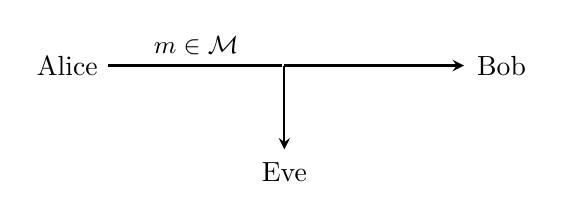
\begin{tikzpicture}[->,>=stealth,shorten >=1pt,auto,node distance=1cm,thick,main node/.style={scale=0.8,circle,draw,font=\sffamily\normalsize}]
                \node[] (1) []{Alice};
                \node[] (x) [right of = 1, xshift = 50]{};
                \node[] (2) [right of = x, xshift = 50]{Bob};
                \node[] (3) [below of = x, yshift = -10]{Eve};

                \path[every node/.style={font=\sffamily\small}]
                    (1) edge[-] node {$m \in \mathcal{M}$} (x.center)
                    (x.center) edge (2)
                    (x.center) edge (3)
                    ;
            \end{tikzpicture}

            \caption{Without an encryption scheme, Eve -- an evildoer -- may be able to read the message that Alice is sending to Bob.}
        \end{figure}

        \item \textbf{Message integrity}: the capability of ensuring that the original message has not been altered even if an outsider intercepts the cyphertext
        
        \begin{figure}[H]
            \centering

            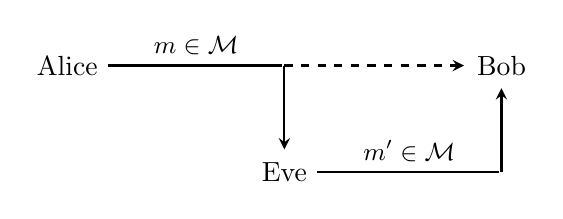
\begin{tikzpicture}[->,>=stealth,shorten >=1pt,auto,node distance=1cm,thick,main node/.style={scale=0.8,circle,draw,font=\sffamily\normalsize}]
                \node[] (1) []{Alice};
                \node[] (x) [right of = 1, xshift = 50]{};
                \node[] (2) [right of = x, xshift = 50]{Bob};
                \node[] (3) [below of = x, yshift = -10]{Eve};
                \node[] (y) [below of = 2, yshift = -10]{};

                \path[every node/.style={font=\sffamily\small}]
                    (1) edge[-] node {$m \in \mathcal{M}$} (x.center)
                    (x.center) edge[dashed] (2)
                    (x.center) edge (3)
                    (3) edge[-] node {$m' \in \mathcal{M}$} (y.center)
                    (y.center) edge (2)
                    ;
            \end{tikzpicture}

            \caption{Without an encryption scheme, Eve may be able to intercept and alter the message that Alice is sending to Bob.}
        \end{figure}
    \end{enumerate}


    Before the 50's, cryptography was considered an \textit{art} for geniouses capable of encrypting and decrypting messages written by other geniouses of the field. In modern days, cryptography became a \textit{mathematical science} with precise definitions and proofs. These mathematical tools separate in two types: \textbf{unconditional proofs} and \textbf{conditional proofs}.
    
    The former type referres to proofs where no assumptions are made, focusing on showing that something is possible without caring about it being inefficient (hence we have theoretically infinite resources at our disposal). The latter, instead, uses real-world assumptions that are believed to be true in order to prove real-world results. The typical example is the $\mathsf{P} \neq \mathsf{NP}$ assumption, i.e. that there are some problems that are verifiable in polynomial time but not solvable in polynomial time. Many cryptosystems are based on the assumption that prime factorization is hard to solve but easy to verify. This is equivalent to assuming that $\mathrm{FACTORING} \in \mathsf{NP} - \mathsf{P}$ (only $\mathrm{FACTORING} \in \mathsf{NP}$ has been proven), making the assumption $\mathsf{P} \neq \mathsf{NP}$ fundamental. Making a crytosystem easy to verify allows us to make it impossible to access a resource without using knowing the solution to the authentication phase.

    \begin{framedthm}{}
        Every cryptosystem based on prime factorization is \curlyquotes{secure} if $\mathrm{FACTORING} \notin \mathsf{P}$
    \end{framedthm}
    
    \begin{proof}[Proof (sketch).]
        By contrapositive, suppose that there is a cryptosystem $\Pi$ that is not \curlyquotes{secure}, meaning that there is a polynomial time algorithm $A$ that is capable of \curlyquotes{breaking} $\Pi$. Then, for each number $n \in \N$ we can forge a message $m$ based on $n$ and use the output $A(m)$ to find the prime factors of $n$, concluding that $\mathsf{FACTORING} \in \mathsf{P}$.
    \end{proof}
    
    These two goals will be discussed under two main types of cryptosystems:
    \begin{itemize}
        \item \textbf{Symmetric cryptography}: both ends of the communication share a single common key that is random and unknown to any outsider.
        \item \textbf{Asymmetric cryptography}: both ends of the communication have each their own key pair $(pk, sk)$ where $pk$ is \textit{public}, i.e. known by everyone, and $sk$ is \textit{secret}, i.e. known only by the owner. 
    \end{itemize}

    Throughout this work we'll use the following notation to talk about cryptographic systems:
    \begin{itemize}
        \item $\mathcal{M}$ is the message space, i.e. the set of all strings of messages that can be sent between two parties.
        \item $\mathcal{C}$ is the cyphertext space, i.e. the set of all strings of cyphertexts that can be produced by a cryptosystem.
        \item $\mathcal{K}$ is the key space, i.e. the set of all strings of keys that can be used in a cryptographic system.
        \item $\mathcal{H}$ is the hashing function space, i.e. the set of all hash functions that can be used by a cryptosystem.
    \end{itemize}

    \chapter{Information-theoretic cryptography}

    \section{Perfect secrecy and Shannon's theorem}

    For now, we'll focus on symmetric cryptography, i.e. cryptosystems where a shared secret key is used for both encryption and decryption. It is widely used due to its speed and efficiency, especially in encrypting large volumes of data. A core model of this approach is \textbf{Secret Key Encryption (SKE)}, which includes three main components:
    \begin{itemize}
        \item A shared \textit{secret key} $K \in_{R} \mathcal{K}$ chosen uniformly at random
        \item An \textit{encryption function} $\mathrm{Enc} : \mathcal{K} \times \mathcal{M} \to \mathcal{C}$ that transforms plaintext into cyphertext
        \item A \textit{decryption function} $\mathrm{Dec} : \mathcal{K} \times \mathcal{C} \to \mathcal{M}$ that transforms a cyphertext into plaintext
    \end{itemize}

    In order to be functional, SKEs must be \textbf{correct}, meaning that if a message $m \in \mathcal{M}$ gets encrypted with $K \in_R \mathcal{K}$ obtaining the cyphertext $c \in \mathcal{C}$, the decryption process over $c$ using the same key $K$ must give back the original message.

    \begin{frameddefn}{Correctness in SKEs}
        An SKE $\Pi = (\mathrm{Enc}, \mathrm{Dec})$ is said to be correct if $\forall m \in \mathcal{M}, \forall K \in_R \mathcal{K}$ it holds that:
        \[\mathrm{Dec}(K, \mathrm{Enc}(K, m)) = m\]
    \end{frameddefn}

    \begin{figure}[H]
        \centering

        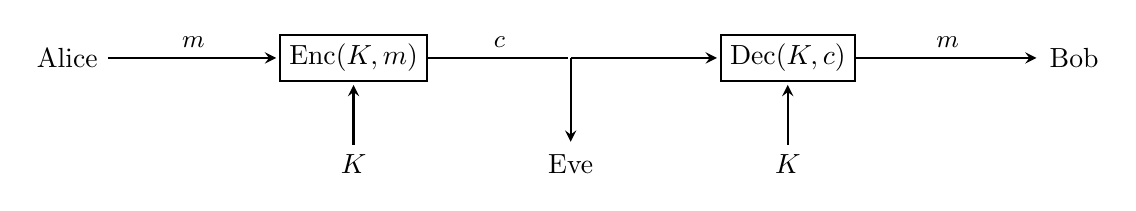
\begin{tikzpicture}[->,>=stealth,shorten >=1pt,auto,node distance=1cm,thick,main node/.style={scale=0.8,circle,draw,font=\sffamily\normalsize}]
            \node[] (1) []{Alice};
            \node[draw, rectangle, minimum width=40] (2) [right of = 1, xshift = 75]{$\mathrm{Enc}(K,m)$};
            \node[] (x) [right of = 2, xshift = 50]{};
            \node[draw, rectangle, minimum width=40] (3) [right of = x, xshift = 50]{$\mathrm{Dec}(K,c)$};
            \node[] (4) [right of = 3, xshift = 75]{Bob};
            \node[] (5) [below of = x, yshift = -10]{Eve};
            \node[] (6) [below of = 2, yshift = -10]{$K$};
            \node[] (7) [below of = 3, yshift = -10]{$K$};

            \path[every node/.style={font=\sffamily\small}]
                (1) edge node{$m$} (2)
                (2) edge[-] node{$c$} (x.center)
                (x.center) edge (3)
                (x.center) edge (5)
                (3) edge node{$m$} (4)
                (6) edge (2)
                (7) edge (3)
                ;
        \end{tikzpicture}

        \caption{Example of SKE with perfect secrecy. Even if Eve intercepts the cyphertext, she cannot obtain the original message since she doesn't know the key.}
    \end{figure}

    Originally proposed in the 19th century by the homonym cryptographer, \textbf{Kerckhoffs's principle} is a foundational concept in cryptography which asserts that the security of a cryptographic system should depend \underline{only} on the secrecy of the key. In other words, a system should be secure even if everything about the system is known publicly, except for the secret key. The principle was later succinctly restated by Claude Shannon as \curlyquotes{the enemy knows the system}.

    During his work, Shannon also proposed a formal definition of \textbf{perfect secrecy}, i.e. a property that fully respects the concept behind Kerckhoff's principle. Shannon's formulation states that the probability of $m$ being the communicated message is equal to the probability of $m$ being the communicated message even when the corresponding cyphertext $c$ is known. In other words, no cyphertext reveals additional information over any message.

    \begin{frameddefn}{Perfect secrecy}
        Let $\Pi = (\mathrm{Enc}, \mathrm{Dec})$ be an SKE. Let $M$ be a random variable over $\mathcal{M}$ and let $C$ be another random variable defined as $C = \mathrm{Enc}(K,M)$, for some key $K \in_R \mathcal{K}$. We say that $\Pi$ has perfect secrecy when $\forall m \in \mathcal{M}$ and $\forall c \in \mathcal{C}$ it holds that:
        \[\Pr[M = m] = \Pr[M = m \mid C = c]\]
    \end{frameddefn}
    
    Shannon proved that such definition is achievable by some cryptosystems, but it comes with inheritent practical limitations. Suprisingly, even a simple SKE as the \textbf{One Time Pad (OTP)} system has perfect secrecy. In this system we assume that everything is a binary string of the same length, i.e. that $\mathcal{M} = \mathcal{K} = \mathcal{C} = \{0,1\}^n$ for some $n \in \N$. The encryption and decryption functions are defined as follows:
    \[\mathrm{Enc}(K, m) = K \oplus m \qquad\qquad \mathrm{Dec}(K,c) = K \oplus c\]
    
    By properties of the bit-wise XOR function, it's easy to see that OTP is complete:
    \[\mathrm{Dec}(K,\mathrm{Enc}(K,m)) = K \oplus (K \oplus m) = m\]

    In order to prove that OTP has perfect secrecy, we start by proving two equivalent definitions of perfect secrecy. In particular, states that for every pair of messages every cyphertext has the same probability of being the output of the encoding function when applied of both messages. 

    \begin{framedlem}[label={perfect_secrecy}]{Perfect secrecy (eq. definitions)}
        Let $\Pi = (\mathrm{Enc}, \mathrm{Dec})$ be an SKE. Let $M$ be a random variable over $\mathcal{M}$ and let $C$ be another random variable defined as $C = \mathrm{Enc}(K,M)$, for some key $K \in_R \mathcal{K}$. The following statements are equivalent:
        \begin{enumerate}
            \item $\Pi$ has perfect secrecy
            \item $M$ and $C$ are independent
            \item $\forall m, m' \in \mathcal{M}$ and $\forall c \in \mathcal{C}$ it holds that:
            \[\Pr_{K \in_R \mathcal{K}}[\mathrm{Enc}(K,m) = c] = \Pr_{K \in_R \mathcal{K}}[\mathrm{Enc}(K,m') = c]\]
        \end{enumerate}
    \end{framedlem}

    \begin{proof}
        \begin{enumerate}
            \item[1. $\implies$ 2.] Suppose that $\Pi$ has perfect secrecy. Then, through definition of conditional probability we get that:
            \[\Pr[M = m] = \Pr[M = m \mid C = c] = \frac{\Pr[M = m, C = c]}{\Pr[C = c]}\]
            which implies that:
            \[\Pr[M = m] \cdot \Pr[C = c] = \Pr[M = m, C = c]\]
            concluding that $M$ and $C$ are independent

            \item Suppose that $M$ and $C$ are independent. Fix $m, m' \in \mathcal{M}$ and $c \in \mathcal{C}$. Through event manipulation and independency of $M$ and $C$ we obtain that:
            \[\begin{split}
                \Pr_{K \in_R \mathcal{K}}[\mathrm{Enc}(K,m) = c] &= \Pr_{K \in_R \mathcal{K}}[\mathrm{Enc}(K,M) = c \mid M = m] \\
                &= \Pr_{K \in_R \mathcal{K}}[C = c \mid M = m]\\
                &= \Pr_{K \in_R \mathcal{K}}[M = m]\\
            \end{split}\]

            Since every message has the same probability of being correct -- without additional information -- we know that:
            \[Pr_{K \in_R \mathcal{K}}[M = m] = Pr_{K \in_R \mathcal{K}}[M = m']\]

            Moreover, through a similar argument to the one above we get that:
            \[\Pr_{K \in_R \mathcal{K}}[\mathrm{Enc}(K,m') = c] = \Pr_{K \in_R \mathcal{K}}[M = m']\]

            \item Assume the third statement holds and fix $c \in \mathcal{C}$
            
            \textbf{Claim}: $\Pr[C = c] = \Pr[C = c \mid M = m]$

            \begin{proof}[Proof of the claim]
                Through the probability sum principle, we get that:
                \[\begin{split}
                    \Pr[C = c] &= \sum_{m' \in \mathcal{M}} \Pr[C = c, M = m] \\
                    &= \sum_{m' \in \mathcal{M}} \Pr[C = c \mid M = m'] \cdot \Pr[M = m'] \\
                    &= \sum_{m' \in \mathcal{M}} \Pr[\mathrm{Enc}(K,M') = c \mid M = m'] \cdot \Pr[M = m'] \\
                    &= \sum_{m' \in \mathcal{M}} \Pr[\mathrm{Enc}(K,m') = c] \cdot \Pr[M = m'] \\
                \end{split}\]

                Through the hypothesis we also get that:
                \[\begin{split}
                    \Pr[C = c] &= \sum_{m' \in \mathcal{M}} \Pr[\mathrm{Enc}(K,m') = c] \cdot \Pr[M = m'] \\
                    &= \sum_{m' \in \mathcal{M}} \Pr[\mathrm{Enc}(K,m) = c] \cdot \Pr[M = m'] \\
                    &= \Pr[\mathrm{Enc}(K,m) = c] \cdot \sum_{m' \in \mathcal{M}} \Pr[M = m'] \\
                    &= \Pr[\mathrm{Enc}(K,m) = c] \cdot 1\\
                    &= \Pr[\mathrm{Enc}(K,M) = c \mid M = m]\\
                    &= \Pr[C = c \mid M = m]\\
                \end{split}\]
            \end{proof}

            By definition of conditional probability, we know that:
            \[ \Pr[M = m \mid C = c] \cdot \Pr[C = c] = \Pr[M = m, C = c] = \Pr[C = c \mid M = m] \cdot \Pr[M = m]\]
            
            which implies that:
            \[\Pr[M = m] = \frac{\Pr[M = m \mid C = c] \cdot \Pr[C = c]}{\Pr[C = c \mid M = m]}\]

            Finally, through the claim we conclude that:
            \[\Pr[M = m] = \frac{\Pr[M = m \mid C = c] \cdot \Pr[C = c]}{\Pr[C = c \mid M = m]} = \Pr[M = m \mid C = c]\]
        \end{enumerate}
    \end{proof}

    \begin{framedprop}{}
        OTP has perfect security.
    \end{framedprop}

    \begin{proof}
        We'll prove that the third definition of \Cref{perfect_secrecy} holds for OTP. Fix two messages $m,m' \in \mathcal{M}$ and a cyphertext $c \in \mathcal{C}$. Through definition of the OTP system and by the properties of the XOR function, we have that:
        \[\Pr_{K \in_R \mathcal{K}}[\mathrm{Enc}(K, m) = c] = \Pr_{K \in_R \mathcal{K}}[K \oplus m = c] = \Pr_{K \in_R \mathcal{K}}[K = m \oplus c] = 2^{-n}\]
        
        Through the same argument, we also get that:
        \[\Pr_{K \in_R \mathcal{K}}[\mathrm{Enc}(K, m') = c] = 2^{-n}\]
    \end{proof}

    We'll now show the inheritent limitations of perfect secrecy. The key idea is simple: in order for $M$ and $C$ to be independent, the key cannot be shorter than the message. Otherwise, there will be some cyphertexts that are unreachable by some messages, revealing information on the system.

    \begin{framedthm}{Shannon's perfect secrecy theorem}
        Let $\Pi = (\mathrm{Enc}, \mathrm{Dec})$ be a non-trivial perfectly secret SKE. Then, it holds that $\abs{\mathcal{K}} \geq \abs{\mathcal{M}}$
    \end{framedthm}

    \begin{proof}
        Suppose that $\Pi$ is a non-trivial perfectly secret. Fix any $c \in \mathcal{C}$ such that $\Pr[C = c] > 0$ (this is where non-triviality is required). Let $\mathcal{M}'$ be the set of possible decryptions over $c$, i.e. $\mathcal{M}' = \{\mathrm{Dec}(K,c) \mid K \in \mathcal{K}\}$. We observe that $\mathcal{M}'$ contains at most one decryption for each key (some keys may yield the same decryption). By way of contradiction, suppose that $\abs{\mathcal{K}} < \abs{\mathcal{M}}$. Then, we get that $\abs{\mathcal{M}'} \leq \abs{\mathcal{K}} < \abs{\mathcal{M}}$.

        This implies that $\exists m \in \mathcal{M} - \mathcal{M}'$. Thus, there is a message that cannot be the result of applying the decryption function on $c$, meaning that $\Pr[M = m \mid C = c] = 0$. However, we know that, when no additional information is given, every message is uniform, hence $\Pr[M = m] = \frac{1}{\mathcal{M}}$, contradicting the fact that $\Pi$ has perfect secrecy.
    \end{proof}

    \section{Message authentication codes}

    We'll now focus on the second key goal of cryptography: \textit{message integrity}. The simplest way to reach such goal is through \textbf{Message Authentication Codes (MACs)}, an additional piece of information sent with the message that enables the receiver to assert that the message hasn't been altered.
    
    For now, we'll start with a simple model that \underline{doesn't care} about secrecy, but only about integrity. This type of MACs use a deterministic \textbf{tagging function} (usually implemented as an \textit{hash function}) $\mathrm{Tag} : \mathcal{K} \times \mathcal{M} \to \mathcal{T}$, where $\mathcal{T}$ is the tag space, i.e. the set of all tag strings.

    \begin{figure}[H]
        \centering

        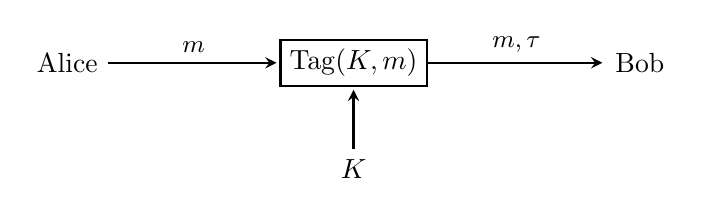
\begin{tikzpicture}[->,>=stealth,shorten >=1pt,auto,node distance=1cm,thick,main node/.style={scale=0.8,circle,draw,font=\sffamily\normalsize}]
            \node[] (1) []{Alice};
            \node[draw, rectangle, minimum width=40] (2) [right of = 1, xshift = 75]{$\mathrm{Tag}(K,m)$};
            \node[] (4) [right of = 2, xshift = 75]{Bob};
            \node[] (6) [below of = 2, yshift = -10]{$K$};

            \path[every node/.style={font=\sffamily\small}]
                (1) edge node{$m$} (2)
                (2) edge node{$m,\tau$} (4)
                (6) edge (2)
                ;
        \end{tikzpicture}

        \caption{Example of an integrity-only MAC.}
    \end{figure}

    The idea behind tagging functions is simple: once the message and the tag have been received, Bob can re-compute the tag using the same key-message pair and compare it to the received tag. If the two tags are equal, Bob is sure that the message hasn't been altered. However, this simple idea can only work under the assumption of \textbf{unforgeability}: 
    \begin{itemize}
        \item It should be hard to forge a valid tag $\tau$ for a message $m$ when the key $K$ is not known
        \item It should be hard to forge a valid tag $\tau$ for a message $m$ even when a pair $(m',\tau')$ is known
    \end{itemize}

    In other words, unforgeability states that no pair should reveal no information about how the tags are computed. Without this property, an adversarial entity may be able to infer information on the shared key and/or the tagging function, using them to forge valid tags. If an entity is capable of forging a valid tag, it may intercept the message-tag pair, alter the message, forge a valid tag for the new message and send a new pair, fooling the receiver. We give a formal definition of a property that reflects this unforgeability aspect.

    \begin{frameddefn}{$t$-time $\varepsilon$-statistical security}
        We say that a MAC $\Pi = (\mathrm{Tag})$ has $t$-time $\varepsilon$-statistical security when $\forall m, m_1, \ldots, m_t \in \mathcal{M}$ and $\forall \tau, \tau_1,\ldots, \tau_t \in\mathcal{T}$, where $m \neq m_i$ and $m_i \neq m_j$ for each $i \neq j$, it holds that:
        \[\Pr_{K \in_R \mathcal{K}} [\mathrm{Tag}(K,m) = \tau \mid \mathrm{Tag}(K,m_1) = \tau_1, \ldots, \mathrm{Tag}(K,m_t) = \tau_t] \leq \varepsilon\]
    \end{frameddefn}

    In simple terms, the above property states that, even when $t$ message-tag pairs $(m_1, \tau_1), \ldots,$ $(m_t, \tau_t)$ are known, the probability of a message-tag pair $(m,\tau)$ being possible is at most $\varepsilon$. Optimally, we want $\varepsilon$ to be as small as possible and $t$ to be as large as possible. However, it's easy to see that $\forall t \in \N$ it is impossible to get $\varepsilon = 0$ since a random $\tau \in \mathcal{T}$ always has probability at least $\frac{1}{\abs{\mathcal{T}}}$ of being correct. Just as we did with perfect secrecy, we'll show that the notion of good statistical security is achievable, but it's highly inefficient in terms of key size. 

    \begin{framedthm}{}
        Any $t$-time $2^{-\lambda}$-statistically secure MAC must have a key of size $(t+1)\lambda$
    \end{framedthm}

    \begin{proof}
        Omitted.
    \end{proof}

    A good enough $1$-time statistically secure MAC is achievable through \textbf{pairwise independent hash functions}, i.e. a family of hash functions where each pair of functions forms a pair of independent random variables. This idea can also be expressed through joint uniform distributions, as in the below definition.

    \begin{frameddefn}{Pairwise independent hash functions}
        Let $\mathcal{H} = \{h_K : \mathcal{M} \to \mathcal{T}\}_{K \in \mathcal{K}}$ be a family of hash functions. We say that $\mathcal{H}$ is pairwise independent if $\forall m, m' \in \mathcal{M}$ with $m \neq m'$ it holds that the distribution $(h_K(m), h_K(m'))$ is uniform over $\mathcal{T} \times \mathcal{T}$ when $K \in_R \mathcal{K}$.

        \textit{Note}: $h_K(m)$ and $h_K(m')$ denote two random variables in this context.
    \end{frameddefn}

    \begin{framedthm}{}
        Let $\mathcal{H} = \{h_K : \mathcal{M} \to \mathcal{T}\}_{K \in \mathcal{K}}$ be a family of pairwise indepependent hash functions induces a $1$-time $\frac{1}{\abs{\mathcal{T}}}$-statistically secure MAC.
    \end{framedthm}

    \begin{proof}
        Fix $m \in \mathcal{M}$ and $\tau \in \mathcal{T}$. Let $\Pi = (\mathrm{Tag})$ be the MAC defined as $\mathrm{Tag}(K,m) = h_K(m)$. Since the joint probability of each pair of hash functions in $\mathcal{H}$ is pairwise uniformly distributed, we get that each hash function is also individually uniformly distributed. Hence, we derive that:
        \[\Pr[\mathrm{Tag}(K,m) = \tau] = \Pr[h_K(m) = \tau] = \frac{1}{\abs{\mathcal{T}}}\]

        Similarly, by pairwise independence $\forall m, m' \in \mathcal{M}$ with $m \neq m'$ and $\forall \tau, \tau' \in \mathcal{T}$ it holds that:
        \[\begin{split}
            \Pr_{K \in_R \mathcal{K}}[\mathrm{Tag}(K,m') = \tau', \mathrm{Tag}(K,m) = \tau] &= \Pr_{K \in_R \mathcal{K}}[\mathrm{Tag}(K,m') = \tau'] \cdot \Pr_{K \in_R \mathcal{K}}[\mathrm{Tag}(K,m) = \tau] \\
            &= \Pr_{K \in_R \mathcal{K}}[h_K(m') = \tau'] \cdot \Pr_{K \in_R \mathcal{K}}[h_K(m) = \tau] \\
            &= \frac{1}{\abs{\mathcal{T}}} \cdot \frac{1}{\abs{\mathcal{T}}}
        \end{split}\]

        Putting the two results together we get that:
        \[\Pr[\mathrm{Tag}(K,m') = \tau' \mid \mathrm{Tag}(K,m) = \tau] = \frac{\Pr_{K \in_R \mathcal{K}}[\mathrm{Tag}(K,m') = \tau', \mathrm{Tag}(K,m) = \tau]}{\Pr[\mathrm{Tag}(K,m) = \tau]} = \frac{1}{\abs{\mathcal{T}}}\]
    \end{proof}

    After proving that pairwise independent hash function families form a good enough MAC, we're left with proving that such families exist. Suprisingly, these families can be easily constructed through prime numbers.
    
    \begin{framedprop}{}
        Given a prime $p \in \Primes$, let $\mathcal{M} = \mathcal{T} = \Z_p$ and $\mathcal{K} = \Z_p^2$. Then, the family $\mathcal{H} = \{h_{(a,b)}\}_{(a,b) \in \Z_p^2}$ where $h_{(a,b)}(m) = am+b \pmod{p}$ is pairwise independent.
    \end{framedprop}

    \begin{proof}
        Fix $m, m' \in \Z_p$ with $m \neq m'$ and $\tau, \tau' \in \Z_p$. We'll show that the joint probability over the hash functions is uniform. First, we observe that:
        \[\begin{split}
            \Pr_{(a,b) \in_R \Z_p^2}[h_{(a,b)}(m) = \tau, h_{(a,b)}(m') = \tau']
            &= \Pr_{(a,b) \in_R \Z_p^2}[am+b = \tau, am' + b = \tau'] \\
            &= \Pr_{(a,b) \in_R \Z_p^2}\sbk{\rmat{m & 1 \\ m' & 1}\rmat{a \\ b} = \rmat{\tau \\ \tau'}}
        \end{split}\]

        Since $m \neq m'$, we know that $\det\rmat{m & 1 \\ m' & 1} = m-m' \neq 0$, thus the matrix is invertible. This allows us to further manipulate the event and rewrite it in terms of the key:
        \[\begin{split}
            \Pr_{(a,b) \in_R \Z_p^2}[h_{(a,b)}(m) = \tau, h_{(a,b)}(m') = \tau']
            &= \Pr_{(a,b) \in_R \Z_p^2}\sbk{\rmat{m & 1 \\ m' & 1}\rmat{a \\ b} = \rmat{\tau \\ \tau'}} \\
            &= \Pr_{(a,b) \in_R \Z_p^2}\sbk{\rmat{a \\ b} = \rmat{m & 1 \\ m' & 1}^{-1} \rmat{\tau \\ \tau'}} \\
            &= \frac{1}{\abs{\Z_p^2}}
        \end{split}\]

        concluding that $\mathcal{H}$ is pairwise independent.
    \end{proof}

    \section{Randomness extraction}

    We discussed how randomness can be used to generate secret keys over a probability distribution, but how a random value be generated? As we will discuss later, randomness is a \underline{crucial} concept for secure cryptography. Clearly, there is no such concept as \textit{real randomness}: even if the whole universe may appear chaotic, everything is technically deterministic. The process of generating a random-enough value is called \textbf{randomness extraction} and it is typically achieved by measuring physical quantities (noise, air humidity, \dots) in order to produce a short unpredictable sequence of bits (e.g. 256 bits), which is expensive to generate and not necessarly uniform. This short \curlyquotes{truly random} sequence gets usually expanded to any desired length -- as long as it is polynomial with respect to the original lenght -- through the use of a \textbf{pseudorandom generator (PRG)}. However, this process requires some strict computational assumptions, which we'll discuss later.
    
    For now, we'll focus on understanding how to extract randomness from an unpredictable secure variable $X$. The first \textbf{extractor} that sparked the idea is Von Neumann's Extractor, which yields a fair random coin from an unpredictable unfair one. Let $B \in \{0,1\}$ be the random variable describing the unpredictable unfair coin, where $\Pr[B = 0] = p < \frac{1}{2}$. Let $Y \in \{0,1\}$ be the random variable describing our new coin. The value of $Y$ is determined by the following procedure. Sample two values $b_1, b_2$ from $B$ at different times. If $b_1 = b_2$, $Y$ assumes no value (marked as $Y = ?$) and we repeat the sampling process. If not, $Y = 1$ if $b_1 = 0$ and $b_2 = 1$, otherwise $Y = 0$ if $b_1 = 1$ and $b_2 = 0$.

    If the sampling process succeeds, i.e. $Y$ assumes a value, we have that $\Pr[Y = 0] = p(1-p)$ and $\Pr[Y = 1] = (1-p)p$, thus $\Pr[Y = 0] = \Pr[Y = 1]$. Moreover, we observe that the probability of $Y= = \, ?$ being true for $m$ consecutive tries is at most:
    \[\Pr[Y = ? \text{ for $m$ tries}] = (\Pr[Y= = \, ?])^m = (1-\Pr[Y = 0 \cup Y = 1])^m \leq (1-2p(1-p))^m\] 

    As $m$ grows to infinity, the latter probability goes to 0, making the even negligible. Implying that $\Pr[Y=0]$ and $\Pr[Y = 1]$ tend to be $\frac{1}{2}$ due to them having the same probability and them being the only two outcomes. This makes $Y$ a fair enough coin.

    Our goal is to generalize this concept to any desider value, i.e. design an extractor $\mathrm{Ext}$ that uses a random variable $X$ to output any desided uniform distribution $\mathrm{Ext}(X)$. A good eye may recognize that this is clearly impossible to achieve unless the source is already truly unpredictable, which makes the extractor useless since we already have a truly random source. As for many computational and probabilistic concepts, we can only hope to achieve something that is good-enough for our purposes. This goodness is measured through a concept known as \textbf{min-entropy}, that being the largest value $m$ having the property that each observation of $X$ provides at least $m$ bits of information.

    \begin{frameddefn}{Min-entropy}
        Given a random variable $X$, we define the min-entropy of $X$ as:
        \[H_{\infty}(X) = - \log \max_{x} \Pr[X = x]\]
    \end{frameddefn}

    One way to justify the name of the quantity is to compare it with the more standard definition of \textit{entropy}, defined as the expectation value of $\log\rbk{\frac{1}{p_i}}$ over a distribution $P$
    \[H(P) = \sum_{i} p_i \log\rbk{\frac{1}{p_i}}\]

    In the min-entropy, instead, we take take the minimum value of $\log\rbk{\frac{1}{p_i}}$, where:
    \[\min_i \log\rbk{\frac{1}{p_i}} = \log \rbk{\min_i \frac{1}{p_i}} = - \log \max_i p_i\]

    Consider a random variable $X \sim U_n$, where $U_n$ is an uniform distribution over $\{0,1\}^n$. In this case, we have that $\Pr[X = x] = 2^{-n}$ for all value $x$ assumable by $X$. Hence, the min-entropy is:
    \[H_{\infty}(X) = -\log \max_x \Pr[X = x] = - \log (2^{-n}) = n\]

    This concludes that each observation of $X$ provides at least $n$ bits of information. Consider now a constant random variable $X'$, i.e. $\Pr[X' = x^*] = 1$ for some fixed value $x^*$ and $\Pr[X' = x] = 0$ for every $x^* \neq x$. It's easy to see that:
    \[H_{\infty}(X') = -\log \max_{x'} \Pr[X' = x] = -\log 1 = 0\]

    Concluding that each observation of $X'$ provides at least 0 bits of information. This information-theoretic measure opens a new question regarding extractors: is there an extractor $\mathrm{Ext}^*$ that for any random variable $X$ outputs an uniform distribution $Y = \mathrm{Ext}(X)$ such that $H_{\infty}(X) \geq k$ for some value $k > 0$? Even under these constraints, the answer to this question is still negative. In particular, it's impossible to define such extractor even if we restrict our interest to extracting only one bit while revealing at least one bit less than the input length.
    
    \begin{framedprop}{}
        There is no extractor $\mathrm{Ext}$ such that for every random variable $X$ over $\{0,1\}^n$ with $H_{\infty}(X) \geq n-1$ it holds that $\mathrm{Ext}(X)$ is a uniform distribution over $\{0,1\}$.
    \end{framedprop}

    \begin{proof}
        Let $\mathrm{Ext} : \{0,1\}^n \to \{0,1\}$ be any extractor and let $b \in \{0,1\}$ be the output maximizing the cardinality of the preimage of the extractor, i.e. the set of inputs for which the extractor outputs $b$.
        \[b = \argmax_{b' \in \{0,1\}} \abs{\mathrm{Ext}^{-1}(b)}\]

        By the pidgeonhole principle, we have that $\abs{\mathrm{Ext}^{-1}(b)} \geq \frac{\abs{\{0,1\}^n}}{2} = 2^{n-1}$. Let $X$ be a random variable uniform over $\mathrm{Ext}^{-1}(b)$. Since $X$ is uniform, we have that $H_{\infty}(X) \geq n-1$. However, we know that $\mathrm{Ext}(X)$ isn't uniform due to the output being always $b$. This concludes that any extractor has always a bad input uniform random variable $X$ that returns a non-uniform distribution $\mathrm{Ext}(X)$.
    \end{proof}

    Since we can't define an extractor that yields an uniform distribution, the best we can hope for is a distribution that is close enough to an uniform one. We use a standard measure for distribution similarity, called \textbf{$\varepsilon$-closeness}.

    \begin{frameddefn}{$\varepsilon$-closeness}
        Let $X,X'$ be two random variables defined over the same set. We say that $X$ and $X'$ are $\varepsilon$-close, written as $X \sim_\varepsilon X'$ when their \textit{statistical distance} $\mathrm{SD}(X; X')$ is at most $\varepsilon$, where:
        \[\mathrm{SD}(X; X') = \frac{1}{2} \sum_{x} \abs{\Pr[X=x] - \Pr[X'=x]}\]
    \end{frameddefn}

    The concept of $\varepsilon$-closeness between two random variables is equivalent to saying that every \textit{unbounded adversary} $A$, i.e. an entity with unlimited computational power that wants to break our system, cannot distinguish whether a value $x$ has been sampled from $X$ or $X'$.
    \[\abs{\Pr[A(x) = 1 : x \in_R X] - \Pr[A(x) = 1 : x \in_R X']} \leq \varepsilon\]
    
    \begin{frameddefn}{Deterministic extractor}
        Let $S$ be a random variable, referred to as \textit{seed}. We say that $\mathrm{Ext} : \{0,1\}^d \times \{0,1\}^n \to \{0,1\}^\ell$ is a $(k,\varepsilon)$-extractor if for every random variable $X$ with $H_{\infty}(X) \geq k$ it holds that $(S, \mathrm{Ext}(S,X)) \sim_{\varepsilon} (S, U_\ell)$ when $S \sim U_d$.
    \end{frameddefn}

    We notice that the condition $(S, \mathrm{Ext}(S,X)) \sim_{\varepsilon} (S, U_\ell)$ implies that the seed must be \textit{public}. This requirement is forced in order to avoid trivial extractors such as $\mathrm{Ext}(S,X) = S$. The idea is to use a source of randomness with high min-entropy in order to force that the output of a \curlyquotes{good} hash function is statistically close to uniform -- even if the input seed wasn't. This result is known as the \textbf{left-over hash lemma}.
    
    The goodness of the hash functions is measured in terms of \textbf{low collision probability}, defined as the expected value that a random variable $Y$ over a set $\mathcal{Y}$ and a copy $Y'$ of $Y$, giving two i.i.d (identical and independend distributions) variables, return the same result:
    \[\mathrm{Col}(Y) = \Pr[Y = Y']\]

    In particular, we observe that since $Y$ and $Y'$ are i.i.d. we get that:
    \[\begin{split}
        \mathrm{Col}(Y) &= \Pr[Y = Y'] = \sum_{y \in \mathcal{Y}} \Pr[Y = y, Y' = y] = \sum_{y \in \mathcal{Y}} \Pr[Y = y]^2 \\
    \end{split}\]
    
    Before proving the left-over hash lemma, we prove the following relationship commonly used in statistical analysis.

    \begin{framedprop}{}
        Let $Y$ be a random variable over a set $\mathcal{Y}$ and assume $\mathrm{Col}(Y) = \frac{1}{\abs{\mathcal{Y}}}(1+4\varepsilon^2)$ for some $\varepsilon \in \R_{> 0}$. Then, it holds that $\mathrm{SD}(Y, U) \leq \varepsilon$, where $U$ is the uniform distribution over $\mathcal{Y}$.
    \end{framedprop}

    \begin{proof}
        We start by observing that:
        \[\mathrm{SD}(Y; U) = \frac{1}{2} \sum_{y \in \mathcal{Y}} \abs{\Pr[Y = y] - \Pr[U = y]} = \frac{1}{2} \sum_{y \in \mathcal{Y}} \abs{\Pr[Y = y] - \frac{1}{\mathcal{Y}}}\]

        For each $y \in \mathcal{Y}$, fix $q_y = \Pr[Y = y] - \frac{1}{\abs{Y}}$ and $s_y = \mathrm{sign}(q_y)$. Let $\vec q = \smat{q_{y_1} & \cdots & q_{y_{\abs{Y}}}}$ and  $\vec s = \smat{s_{y_1} & \cdots & s_{y_{\abs{Y}}}}$. We notice that:
        \[\mathrm{SD} = \frac{1}{2} \sum_{y \in \mathcal{Y}} \abs{\Pr[Y = y] - \frac{1}{\mathcal{Y}}} = \frac{1}{2} \sum_{y \in \mathcal{Y}} q_y s_y = \frac{1}{2} \abk{\vec q, \vec s}\]

        By the \textit{Cauchy-Swartz inequality} (which we won't prove), we get that:
        \[\mathrm{SD}(Y; U) = \frac{1}{2} \abk{\vec q, \vec s} \leq \frac{1}{2} \sqrt{\abk{\vec q, \vec q} \abk{\vec s, \vec s}} = \frac{1}{2} \sqrt{\rbk{\sum_{y \in \mathcal{Y}} q_y^2} \abs{\mathcal{Y}}}\]

        \textbf{Claim}: $\displaystyle \sum_{y \in \mathcal{Y}} q_y^2 \leq \frac{4\varepsilon^2}{\abs{Y}}$

        \begin{proof}[Proof of the claim]
            Through algebraic manipulation we get that:
            \[\begin{split}
                \sum_{y \in \mathcal{Y}} q_y^2 &= \sum_{y \in \mathcal{Y}} \rbk{\Pr[Y = y] - \frac{1}{\mathcal{Y}}}^2 \\
                &= \sum_{y \in \mathcal{Y}} \rbk{\Pr[Y = y]^2 - \frac{2}{\abs{\mathcal{Y}}} \Pr[Y = y] + \frac{1}{\abs{\mathcal{Y}}^2}} \\
                &= \sum_{y \in \mathcal{Y}} \Pr[Y = y]^2 - \sum_{y \in \mathcal{Y}} \frac{2}{\abs{\mathcal{Y}}} \Pr[Y = y] + \sum_{y \in \mathcal{Y}} \frac{1}{\abs{\mathcal{Y}}^2} \\
                &= \sum_{y \in \mathcal{Y}} \Pr[Y = y]^2 - \frac{2}{\abs{\mathcal{Y}}} + \frac{1}{\abs{\mathcal{Y}}} \\
                &= \mathrm{Col}(Y) - \frac{1}{\mathcal{Y}}
            \end{split}\]

            By hypothesis, we know that the collision probability of $Y$ is bounded, concluding that:
            \[\sum_{y \in \mathcal{Y}} q_y^2 = \mathrm{Col}(Y) - \frac{1}{\mathcal{Y}} \leq \frac{1}{\abs{\mathcal{Y}}}(1+4\varepsilon^2) - \frac{1}{\mathcal{Y}} = \frac{4\varepsilon^2}{\abs{\mathcal{Y}}}\]
        \end{proof}

        Through the claim we directly conclude that:
        \[\mathrm{SD}(Y;U) = \frac{1}{2} \sqrt{\rbk{\sum_{y \in \mathcal{Y}} q_y^2} \abs{\mathcal{Y}}} \leq \frac{1}{2} \sqrt{\frac{4\varepsilon^2}{\abs{\mathcal{Y}}} \abs{Y}} = \varepsilon\]
    \end{proof}

    \begin{framedlem}{Left-over hash lemma}
        Let $\mathcal{H} = \{h_S : \{0,1\}^n \to \{0,1\}^\ell\}_{S \in \{0,1\}^d}$ be a pairwise independent hash function. Let $X$ be a random variable with $H_{\infty}(X) \geq k$. Then, for each $S \in \{0,1\}^d$ it holds that $\mathrm{Ext}(S,X) = h_S(X)$ is a $(k,\varepsilon)$-extractor for $k \geq \ell + 2\log \rbk{\frac{1}{\varepsilon}} - 2$
    \end{framedlem}

    \begin{proof}
        Fix $S \in \{0,1\}^d$ and two random variables $X,X'$. Let $Y = (S, \mathrm{Ext}(S,X))$ and let $Y'$ be a copy of $Y$ defined as and $Y' = (S', \mathrm{Ext}(S',X'))$. We observe that:
        \[\begin{split}
            \mathrm{Col}(Y) &= \Pr[Y = Y'] \\
            &= \Pr[S = S', \mathrm{Ext}(S,X) = \mathrm{Ext}(S',X')] \\
            &= \Pr[S = S', h_S(X) = h_{S'}(X')]
        \end{split}\]

        Since $S$ and $S'$ are independend from $X$ and $X'$, we get that:
        \[\begin{split}
            \mathrm{Col}(Y) &= \Pr[S = S', h_S(X) = h_{S'}(X')] \\
            &= \Pr[S = S', h_S(X) = h_S(X')] \\
            &= \Pr[S = S'] \cdot \Pr[h_S(X) = h_{S}(X')] \\
            &= 2^{-d} \cdot \Pr[h_S(X) = h_{S}(X')] \\
            &= 2^{-d} \cdot (\Pr[X = X', h_S(X) = h_{S}(X')] + \Pr[X \neq X', h_S(X) = h_{S}(X')])\\
            &= 2^{-d} \cdot (\Pr[X = X'] + \Pr[X \neq X', h_S(X) = h_{S}(X')])\\
            &= 2^{-d} \cdot (\Pr[X = X'] + 2^{-\ell})\\
        \end{split}\]
        
        By hypothesis, we know that $H_{\infty}(X) \geq k$. This implies that $\Pr[X = X'] \leq 2^{-k}$ since an adversary cannot guess whether a sample comes from $X$ or $X'$ with probability greater than $2^{-k}$.
        \[\begin{split}
            \mathrm{Col}(Y) &= 2^{-d} \cdot (\Pr[X = X'] + 2^{-\ell})\\
            &= 2^{-d} \cdot (2^{-k} + 2^{-\ell})\\
            &= \frac{1}{2^{d+\ell}}(2^{\ell-k} + 1)
        \end{split}\]

        Finally, by hypothesis we have conclude that:
        \[\mathrm{Col}(Y) \leq \frac{1}{2^{d+\ell}}(2^{\ell-k} + 1) \leq \frac{1}{2^{d+\ell}}\rbk{2^{2-2\log \rbk{\frac{1}{\varepsilon}}} + 1} = \frac{4\varepsilon^2 + 1}{\abs{\mathcal{Y}}}\]
    \end{proof}

    \section{Solved exercises}

    \begin{framedprob}{}
        Given a prime $p \in \Primes$, let $\mathcal{M} = \mathcal{T} = \Z_p$ and $\mathcal{K} = \Z_p^2$. Prove that the hash family $\mathcal{H} = \{h_{(a,b)}\}_{(a,b) \in \Z_p^2}$, where $h_{(a,b)}(m) = am+b \pmod{p}$, cannot be a $2$-time statistically secure MAC
    \end{framedprob}

    \textit{Solution}. Suppose that the values $h_{(a,b)}(m_1) = \tau_1$ and $h_{(a,b)}(m_2) = \tau_2$, where $m_1 \neq m_2$, are known to an adversary. Hence, the adversary knows that:
    \[\soe{l}{
        am_1 + b \equiv \tau_1 \pmod{p} \\
        am_2 + b \equiv \tau_2 \pmod{p} \\
    } \implies a(m_1-m_2) \equiv \tau_1 - \tau_2 \pmod{p}\]

    Since $m_1 \neq m_2$, the value $m_1 - m_2$ is invertible in $\Z_p$, the value $Q \equiv (\tau_1 - \tau_2)(m_1 - m_2)^{-1} \pmod{p}$ (notice that $a \equiv Q \pmod{p}$) can be easily computed. Once $Q$ is known, $b$ can be easily computed as $b \equiv \tau_1 - Qm_1 \pmod{p}$. Therefore, we have that:
    \[\Pr_{K \in_R \Z_p}[h_K(m) = \tau \mid h_K(m_1) = \tau_1, h_K(m_2) = \tau_2] = \soe{ll}{
        1 & \text{if } \tau \equiv Q(m -m_1)+ \tau_1 \pmod{p} \\
        0 & \text{otherwise}
    }\]
    
    making $\mathcal{H}$ statistically insecure for every value $0 < \varepsilon < 1$.

    \begin{framedprob}{}
        Construct a 3-wise independent hash function family and prove it's correctness.
    \end{framedprob}

    \textit{Solution}. Given a prime $p \in \Primes$, let $\mathcal{M} = \mathcal{T} = \Z_p$ and $\mathcal{K} = \Z_p^3$. Consider the hash family $\mathcal{H} = \{h_{(a,b,c)}\}_{(a,b,c) \in \Z_p^2}$, where $h_{(a,b,c)}(m) = am^2+bm+c \pmod{p}$.

    Fix three values $x_1, x_2, x_3 \in \Z_p$ such that $x_i \neq x_j$ for all $i \neq j$. Fix $\tau_1, \tau_2, \tau_3 \in \Z_p$. We observe that:
    \[\begin{split}
        \Pr_{(a,b,c) \in_R \Z_p^3}\smat{\begin{array}{c}
            h_{(a,b,c)}(x_1) = \tau_1\\
            h_{(a,b,c)}(x_2) = \tau_2\\
            h_{(a,b,c)}(x_3) = \tau_3
        \end{array}} &= \Pr_{(a,b,c) \in_R \Z_p^3}\smat{\begin{array}{c}
            ax_1^2+bx_1+c = \tau_1\\
            ax_2^2+bx_2+c = \tau_2\\
            ax_3^2+bx_3+c = \tau_3
        \end{array}}  \\
        &= \Pr_{(a,b,c) \in_R \Z_p^3} \sbk{\rmat{x_1^2 & x_1 & 1 \\ x_2^2 & x_2 & 1 \\ x_3^2 & x_3 & 1} \rmat{a \\ c \\ b} = \rmat{\tau_1 \\ \tau_2 \\ \tau_3}}
    \end{split}\]

    Since $x_i \neq x_j$ for all $i \neq j$, we observe that the matrix is invertible:
    \[\begin{split}
        \det \rmat{x_1^2 & x_1 & 1 \\ x_2^2 & x_2 & 1 \\ x_3^2 & x_3 & 1} &= x_1^2 \det \rmat{x_2 & 1 \\ x_3 & 1} - x_2^2 \det \rmat{x_1 & 1 \\ x_3 & 1} + x_3^2 \det \rmat{x_1 & 1 \\ x_2 & 1} \\
        &= x_1^2x_2 - x_1^2x_3 - x_2^2x_1 + x_2^2 x_3 + x_3^2 x_1 - x_3^2x_2 \\
        &= (x_1-x_2)(x_1-x_3)(x_2-x_3) \\
        &\neq 0
    \end{split}\]

    concluding that $\mathcal{H}$ is 3-wise independent:

    \[\begin{split}
        \Pr_{(a,b,c) \in_R \Z_p^3}\smat{\begin{array}{c}
            h_{(a,b,c)}(x_1) = \tau_1\\
            h_{(a,b,c)}(x_2) = \tau_2\\
            h_{(a,b,c)}(x_3) = \tau_3
        \end{array}} &= \Pr_{(a,b,c) \in_R \Z_p^3} \sbk{\rmat{x_1^2 & x_1 & 1 \\ x_2^2 & x_2 & 1 \\ x_3^2 & x_3 & 1} \rmat{a \\ c \\ b} = \rmat{\tau_1 \\ \tau_2 \\ \tau_3}}\\
        &= \Pr_{(a,b,c) \in_R \Z_p^3} \sbk{\rmat{a \\ c \\ b} = \rmat{x_1^2 & x_1 & 1 \\ x_2^2 & x_2 & 1 \\ x_3^2 & x_3 & 1}^{-1} \rmat{\tau_1 \\ \tau_2 \\ \tau_3}} \\
        &= \frac{1}{\abs{\Z_p^3}}
    \end{split}\]

    \chapter{Computational security}

    \section{One-way functions and Impagliazzo's worlds}

    In the previous chapter we discussed how, without computational assumptions, symmetric encryption and random generation can be achieved with some strong limitations. For privacy and integrity, we saw how the message length and the key length must be at least equal in order to guarantee a 1-time security (no guarantees for $t$-time security with $t > 1$). For randomness, instead, we saw how we can't extract more than $k$ bits when the min-entropy is $k$.

    Our next objective is to overcome all these limitation (or at least reduce them). This can be achieved at the price of two very strong assumptions:
    \begin{enumerate}
        \item The adversary is \textit{computationally bounded}, i.e. it has limited resources
        \item There are \textit{hard} problems
    \end{enumerate} 
    
    In other words, we'll prove results of the following form. \curlyquotes{if problem $X$ is hard against efficient solvers then cryptosystem $\Pi$ is secure against efficient adversary}. The direct consequence of these results is their contrapositive: if the system $\Pi$ were ever to be proved insecure, there would be an efficient solution for problem $X$. Depending on the \curlyquotes{level of hardness} of problem $X$, this would have groundbreaking consequences (e.g. $X$ could be a problem that implies $\mathsf{P} = \mathsf{NP}$, factoring is easy, discrete-log is easy, \dots).

    Someone may ask \curlyquotes{can't we just assume that $\mathsf{P} \neq \mathsf{NP}$ and prevent all of this?} The answer is \textit{yes}, we could, but this assumption would be \textit{too weak} for our necessities. In fact, to achieve \underline{good security} we require something that isn't directly implied by $\mathsf{P} \neq \mathsf{NP}$: the existence of \textbf{one-way functions (OWF)}. In simple terms, a functions $f : \{0,1\}^n \to \{0,1\}^m$ is said to be \textit{one-way} when it can be efficiently computed but hard to invert (meaning that $f^{-1}$ cannot be efficiently computed).
    
    It's easy to see that assuming the existence of OWFs implies that $\mathsf{P} \neq \mathsf{NP}$. This is due to the contrapositive statement: if $\mathsf{P} = \mathsf{NP}$ then OTWs cannot exist since for each function $f$ we can efficiently verify if $f(x) = y$ in order to compute $f^{-1}(y) = x$. However, the converse statement doesn't hold: assuming $\mathsf{P} \neq \mathsf{NP}$ could still imply that OWFs don't exist. In the article \href{https://dx.doi.org/10.1109/SCT.1995.514853}{A Personal View of Average-Case Complexity} presented at the 1995 Complexity Conference, Russell Impagliazzo describes \textbf{five possible worlds} that we may be living in and their implications to computer science:
    \begin{itemize}
        \item \textit{Algorithmica}: there are no hard problems ($\mathsf{P} = \mathsf{NP}$) and OWFs cannot exist.
        \item \textit{Heuristica}: there are hard problems ($\mathsf{P} \neq \mathsf{NP}$) but can they solved efficiently on average
        \item \textit{Pessiland}: there are hard problems ($\mathsf{P} \neq \mathsf{NP}$) but OWFs don't exist
        \item \textit{Minicrypt}: one-way functions exist but public-key cryptography is impossible 
        \item \textit{Cryptomania}: one-way functions exist and public-key cryptography is possible
    \end{itemize}

    Impagliazzo does not guess which world we live in, but describes \textit{Pessiland} as the worst one out of all possible worlds: in this scenario, not only can we not solve hard problems on average but we apparantly do not get any cryptographic advantage from the hardness of these problems. Today, most computer scientists believe (and hope) that our world corresponds to either \textit{Cryptomania} or \textit{Minicrypt}.

    All the results will be discussed with respect to a fixed standard computational model: the \textit{Turing machine} (TM). From now on, \textit{efficient computation} will refer to a computation made under a polynomial amount of steps with respect to the input size, i.e. if the input $x$ has length $n$ then $\poly(n)$-time referres to at most $n^{c}$ steps, for some $c \in \N$.
    
    As mentioned before, the adversary we'll also assume that the adversary has limited resources. However, we'll be generous with them: the adversary is allowed to use a $\poly(n)$ amount of time and a $\poly(n)$ amount of \textit{random bits}. This implies that their computational model is a \textit{probabilistic polynomial time (PPT)} TM. To formally define the concept of OWFs, we'll use \textbf{negligible functions}, i.e. functions $\varepsilon : \N \to \R$ such that $\forall c \in \N$ there is a value $\lambda_0 \in \N$ for which $\forall \lambda > \lambda_0$ it holds that
    \[\varepsilon(\lambda) < \frac{1}{\lambda^c}\]

    \begin{frameddefn}{One-way functions}
        We say that a function $f : \{0,1\}^n \to \{0,1\}^m$ is a one-way function if:
        \begin{itemize}
            \item $f$ is computable in $\poly(n)$-time
            \item for every PPT algorithm $A$ there is a negligible function $\negl(n)$ such that:
            \[\Pr_{x \in_R U_n}[f(x') = y : y = f(x); x' \gets A(y)] \leq \negl(n)\]
        \end{itemize}

        \textit{Note}: $x \gets A(y)$ is read as \curlyquotes{$x$ is the output of $A(y)$}
    \end{frameddefn}

    \section{Pseudorandom generators}

    In the previous chapter we discussed how randomness is essential for good cryptography, even though true randomness cannot be achieved. To get a good enough approximation of true randomness, modern systems use \textbf{pseudo-randomness}, i.e. efficient deterministic algorithms that generate a sequence of bits that look unpredictable but aren't truly random. By definition, if enough time and resources are permitted an adversary is clearly able to learn how a pseudorandom algorithm work through bruteforce. Hence, we'll restrict that our adversary doesn't have such time and resources, i.e. their computation must also be efficient.
    
    The idea behind pseudo-randomness is to generate a \curlyquotes{non-random} probability distribution (this doesn't really mean anything, but you get the idea) that is \textbf{computationally indistinguishable} from a truly random probability distribution. The formal definition of computational indistinguishability refers to \textit{probability ensembles}, i.e. infinite sequences of probability distributions $\mathcal{X} = \{X_n\}_{n \in \N}$, where each $X_n$ is a distribution over $\{0,1\}^n$. This multi-length definition takes into account the fact that the distribution may change over the input length.

    \begin{frameddefn}{Computational indistinguishability}
        Let  $\mathcal{X} = \{X_n\}_{n \in \N}$ and  $\mathcal{Y} = \{Y_n\}_{n \in \N}$ be two probability ensambles. We say that $\mathcal{X}$ and $\mathcal{Y}$ are computationally indistinguishable, written as $\mathcal{X} \approx_c \mathcal{Y}$, if for every PPT algorithm $D$ there is a negligible function $\negl(n)$ such that $\forall n \in \N$ it holds that:
        \[\abs{\Pr[D(z) = 1 : z \in_R X_n] - \Pr[D(z) = 1 : z \in_R Y_n]} \leq \negl(n)\]
    \end{frameddefn}

    We observe that we already discussed a definition similar to the one above when we talked about $\varepsilon$-closeness. In fact, this can be seen as a practical computational counterpart of that definition (notice how the adversary is now restricted to PPT algorithms and the distributions vary over input lengths). Moreover, it's esy to see that the relation $\approx_c$ is \textit{transitive}, i.e. if $\mathcal{X} \approx_c \mathcal{Y}$ and $\mathcal{Y} \approx_c \mathcal{Z}$ then $\mathcal{X} \approx_c \mathcal{Z}$, and closed under \textit{reductions}, i.e. for any PPT function $f$ if $\mathcal{X} \approx_c \mathcal{Y}$ then $f(\mathcal{X}) \approx_c f(\mathcal{Y})$.

    \begin{frameddefn}{Pseudorandom generator (PRG)}
        Let $G : \{0,1\}^n \to \{0,1\}^{n+\ell}$ be a function where $\ell \geq 1$. We say that $G$ is a pseudorandom generator (PRG) with expansion factor $\ell$ if:
        \begin{itemize}
            \item $G$ can be computed in $\poly(n)$-time
            \item $G(U_n) \approx_c U_{n+\ell}$.
        \end{itemize}
    \end{frameddefn}

    The above definition requires a bit of discussion in order to be fully understood. First, we observe that $G$ is \underline{deterministic}, making $G(U_n) \approx_c U_{n+\ell}$ a very strong property. Then, we observe that the idea  a PRG is to generate new bits that look like they are truly random, as long as the initial seed is already truly random (in practice, we use a seed that is computationally indistinguishable from a truly random one). Hence, we can use a randomness extractor to get an initial seed and then pass it to a PRG in order to \curlyquotes{expand the seed} up to any desired length: after constructing a simple PRG $G : \{0,1\}^n \to \{0,1\}^{n+1}$, it can be used to construct a new PRG $G : \{0,1\}^n \to \{0,1\}^{n+\ell}$ up to any polynomial value $\ell > 0$.

    To prove this result, we use a technique known as \textbf{hybrid argument}. We define a sequence $H_0, \ldots, H_\ell$ of distributions such that:
    \begin{itemize}
        \item $H_0 \approx_c G^\ell(U_n)$ and $H_\ell \approx_c U_{n+\ell}$
        \item $H_i \approx_c H_{i+1}$ for each $i \in [0, \ell-1]$
        \item Each $H_i$ is an hybrid of truly random and pseudorandom bits, where the number of truly random bits increases as $i$ grows, getting replacing the pseudorandom bits
    \end{itemize}

    \begin{framedthm}{PRG stretching}
        Let $G : \{0,1\}^n \to \{0,1\}^{n+1}$ be a PRG. Then, for any $\ell = \poly(n)$ there is a PRG $G^\ell : \{0,1\}^n \to \{0,1\}^{n+\ell}$.
    \end{framedthm}

    \begin{proof}
        For each $i \in [0, \ell]$, let $f_i(s) = b_1 \concat \ldots \concat b_\ell \concat s_\ell$ -- where $\concat$ is the string concatenation operator -- be the function computed through the following algorithm (see \Cref{prg_stretching_1}).

        $f_i$ = "On input $s \in \{0,1\}^n$: 
        \begin{enumerate}
            \item Set $s_i = s$
            \item For each $j \leq i$ set $b_j$ as a truly random bit, i.e. $b_j \in_R U_1$
            \item For each $j > i$ set $s_j$ and $b_j$ as the values such that $G(s_{j-1}) = s_j \concat b_j$, where $s_j \in \{0,1\}^n$ and $b_j \in \{0,1\}$."
        \end{enumerate}

        It's easy to see that each $i \in [0,\ell]$ the function $f_i$ is PPT-computable since $G$ is a PPT algorithm by hypothesis and $\ell = \poly(n)$. Moreover, $f_0$ is deterministic since it doesn't generate random bits. Let $H_0, \ldots, H_\ell$ be the distributions over the outputs of the functions $f_0, \ldots, f_\ell$. We observe that $H_\ell = U_{n+\ell}$ since every bit is truly random in $f_\ell$. Hence, by letting $G^\ell = f_0$ we get that $H_0 = G^\ell(U_n)$ and $H_\ell = U_{n+\ell}$.

        \textbf{Claim:} For each $i \in [0,\ell-1]$ it holds that $H_i \approx_c H_{i+1}$.

        \begin{proof}[Proof of the claim.]
            Fix $i \in [0,\ell-1]$. We prove the claim by reducing the distinguishability of $G(U_n)$ from $U_{n+1}$ to the distinguishability of $H_i$ from $H_{i+1}$. By way of contradiction, suppose that $H_i \not\approx_c H_{i+1}$, meaning that there is a distinguisher $D_i$ such that:
            \[\abs{\Pr[D_i(z) = 1 : z \in_R H_i] - \Pr[D_i(z) = 1 : z \in_R H_{i+1}]} > \frac{1}{n^c}\]
            for some $c > 0$. Let $D$ be the algorithm defined as follows:

            $D$ = "On input $w \in \{0,1\}^{n+1}$:
            \begin{enumerate}
                \item Set $s$ and $b$ as the values such that $w = s \concat b$, where $s \in \{0,1\}^n$ and $b \in \{0,1\}$.
                \item Compute $f_{i+1}(s) = b_1 \concat \ldots \concat b_\ell \concat s_\ell$.
                \item Set $z' = b_1 \concat \ldots \concat b_{i-1} \concat \, b\,  \concat b_{i+1} \concat \ldots \concat b_\ell \concat s_\ell$.
                \item Return $D_i(z_w)$."
            \end{enumerate}

            We observe that $H_i$ and $H_{i+1}$ differ from each other only by one bit: in $f_i$, the bit $b_i$ is the last bit of $G(s_{i-1})$, while in $f_{i+1}$ it is a truly random bit. Hence, when $D$ is given an input $w \in G(U_n)$, the last bit of $w$ is generated through $G$, making the string $z'$ built by $D$ an input sampled from $H_i$. Vice versa, when $D$ is given an input $w \in_R U_{n+1}$, the last bit of $w$ is truly random, making the string $z'$ built by $D$ an in input sampled from $H_{i+1}$. Therefore, we get that:
            \[\begin{split}
                &\abs{\Pr[D(w) = 1 : w \in_R G(U_n)] - \Pr[D(w) = 1 : w \in_R U_{n+1}]}\\
                = &\abs{\Pr[D_i(z') = 1 : z' \in_R H_i] - \Pr[D_i(z') = 1 : z' \in_R H_{i+1}]} \\
                > &\frac{1}{n^c}
            \end{split}\]
            concluding that $D$ is a distinguisher for $G$, raising a contradiction over $G$ being a PRG.
        \end{proof}

        By transitivy of $\approx_c$ and the above claim, we conclude that $G^\ell(U_n) = H_0 \approx_c \ldots \approx_c H_\ell = U_{n+\ell}$, meaning that $G^\ell$ is a PRG.
    \end{proof}

    \begin{figure}[H]
        \centering

        \begin{tikzpicture}[->,>=stealth,shorten >=1pt,auto,node distance=1.5cm,thick,main node/.style={scale=0.8,circle,draw,font=\sffamily\normalsize}]
            \node[] (10) []{$f_0:$};
            \node[] (11) [right of = 10, xshift = 20, color = red]{$s_0$};
            \node[rectangle, draw] (12) [right of = 11]{$G$};
            \node[] (13) [right of = 12]{$s_1$};
            \node[rectangle, draw] (14) [right of = 13]{$G$};
            \node[] (15) [right of = 14]{$s_2$};
            \node[rectangle, draw] (16) [right of = 15]{$G$};
            \node[] (17) [right of = 16]{$\cdots$};
            \node[rectangle, draw] (18) [right of = 17]{$G$};
            \node[] (19) [right of = 18]{$s_\ell$};
            \node[] (110) [below of = 12]{$b_1$};
            \node[] (111) [below of = 14]{$b_2$};
            \node[] (112) [below of = 16]{$b_3$};
            \node[] (113) [below of = 18]{$b_\ell$};

            \node[] (20) [below of = 10, yshift = -50]{$f_1:$};
            \node[] (21) [right of = 20, xshift = 20]{};
            \node[] (22) [right of = 21]{};
            \node[] (23) [right of = 22, color = red]{$s_1$};
            \node[rectangle, draw] (24) [right of = 23]{$G$};
            \node[] (25) [right of = 24]{$s_2$};
            \node[rectangle, draw] (26) [right of = 25]{$G$};
            \node[] (27) [right of = 26]{$\cdots$};
            \node[rectangle, draw] (28) [right of = 27]{$G$};
            \node[] (29) [right of = 28]{$s_\ell$};
            \node[] (210) [below of = 22, color = red]{$b_1$};
            \node[] (211) [below of = 24]{$b_2$};
            \node[] (212) [below of = 26]{$b_3$};
            \node[] (213) [below of = 28]{$b_\ell$};

            \node[] (30) [below of = 20, yshift = -50]{$f_2:$};
            \node[] (31) [right of = 30, xshift = 20]{};
            \node[] (32) [right of = 31]{};
            \node[] (33) [right of = 32]{};
            \node[] (34) [right of = 33]{};
            \node[] (35) [right of = 34, color = red]{$s_2$};
            \node[rectangle, draw] (36) [right of = 35]{$G$};
            \node[] (37) [right of = 36]{$\cdots$};
            \node[rectangle, draw] (38) [right of = 37]{$G$};
            \node[] (39) [right of = 38]{$s_\ell$};
            \node[] (310) [below of = 32, color = red]{$b_1$};
            \node[] (311) [below of = 34, color = red]{$b_2$};
            \node[] (312) [below of = 36]{$b_3$};
            \node[] (313) [below of = 38]{$b_\ell$};

            \path[every node/.style={font=\sffamily\small}]
                (11) edge (12)
                (12) edge (13)
                (13) edge (14)
                (14) edge (15)
                (15) edge (16)
                (16) edge (17)
                (17) edge (18)
                (18) edge (19)
                (12) edge (110)
                (14) edge (111)
                (16) edge (112)
                (18) edge (113)

                (23) edge (24)
                (24) edge (25)
                (25) edge (26)
                (26) edge (27)
                (27) edge (28)
                (28) edge (29)
                (24) edge (211)
                (26) edge (212)
                (28) edge (213)

                (35) edge (36)
                (36) edge (37)
                (37) edge (38)
                (38) edge (39)
                (36) edge (312)
                (38) edge (313)
            ;
        \end{tikzpicture}

        \caption{The idea behind the construction of the functions $f_0, \ldots, f_\ell$. Red strings represent truly random bits.}
        \label{prg_stretching_1}
    \end{figure}

    \newpage

    \section{Hard-core predicates}

    In the previous chapter we saw how a PRG with stretch $1$ is -- in theory -- sufficient to construct a PRG with stretch $\mathrm{poly}(n)$. The next natural objective is to build such PRG with stretch $1$.
    In theoretical terms, we'll see that such PRG can be constructed from any OWF. However, it can be proven that the existence of OWF and PRG is equivalent, i.e. that there exists an OWF if and only if there is a PRG. This theoretical result makes building PRG as hard as building a OWF, which we aren't even sure it exists. To bypass (only partially) this problem, in practical applications we build good-enough PRGs using heuristic constructions.

    \begin{framedthm}{From PRGs to OWFs}
        Let $G : \{0,1\}^n \to \{0,1\}^{2n}$ be a PRG. Then, there is a OWF $f : \{0,1\}^{2n} \to \{0,1\}^{2n}$.
    \end{framedthm}

    \begin{proof}
        Let $f$ be the function that runs $G$ on the first half of the input:
        \[f(x_1 \concat \ldots \concat x_{2n}) = G(x_1 \concat \ldots \concat x_n)\]
        
        By way of contradiction, suppose that $f$ is not a OWF, meaning that there is an adversary $A$ such that:
        \[\Pr_{x \in_R U_n}[f(x') = y : y = f(x); x' \gets A(y)] \geq \frac{1}{n^c}\]
        for some $c > 0$. We build an adversary $D$ defined as:

        $D$ = "On input $z \in \{0,1\}^{2n}$:
        \begin{enumerate}
            \item Compute $A(z) = b_1 \concat \ldots \concat b_{2n}$
            \item If $G(b_1 \concat \ldots \concat b_n) = z$ accept, otherwise reject."
        \end{enumerate}

        If $z \in_R U_{2n}$, the adversary $D$ accepts with probability at most $2^{-n}$ since the first half of the output $A(z)$ is also uniform at random. If $z \in_R G(U_{n})$, instead, the adversary $D$ accepts with probability at least $n^{-c}$ since it first inverts the output and then recomputes it to distinguish it. Hence, we conclude that:
        \[\abs{\Pr[D(z) = 1 : z \in_R G(U_n)] - \Pr[D(z) = 1 : z \in_R U_{2n}]} \geq \frac{1}{n^c} - \frac{1}{2^n} \geq \frac{1}{n^c}\]
        contradicting the assumption of $G$ being a PRG.
    \end{proof}

    To prove that the implication also holds from right to left, thus that OWF imply PRGs, we need a fundamental theoretical concept called \textbf{hard-code bits}. Given a function $f$, these bits contain information about an input $x$ that is hard to obtain from the output $f(x)$, meaning that any adversary $A$ cannot do better than guessing with 50\% chance -- up to some negligible error -- if the bit comes from $x$ or not. Hard-core bits are given by a function $h$ -- called \textit{predicate} -- that extract an hard-core bit from any input $x$.

    \begin{frameddefn}{Hard-core predicate}
        Let $f : \{0,1\}^n \to \{0,1\}^m$ be a PPT-computable function. We say that a function $h : \{0,1\}^n \to \{0,1\}$ is a hard-core predicate for $f$ if for every PPT adversary $A$ it holds that:
        \[\Pr[A(y) = h(x) : x \in_R U_n, y = f(x)] \leq \frac{1}{2} + \negl(n)\]
    \end{frameddefn}
    
    From the very definition that we just gave, it's easy to get an equivalent formulation: $h$ is hard-core for $f$ if and only if $(f(x), h(x)) \approx_c (f(x), U_1)$ with $x \in_R U_n$ (proof is left as an exercise).
    
    We observe that both definitions we gave don't require that $f$ is a OWF. However, hard-core predicates are -- intuitively -- what allows a function to be one-way: if we can establish an hard-core bit for every input $x$, any adversary will have a hard time inverting $f(x)$ due to this very bit. From these observation, we ask three questions:
    \begin{enumerate}
        \item Is there a universal hard-core predicate that is hard-core for every OWF?
        \item Is every function with an hard-core predicate also one-way?
        \item Does every one-way function have an hard-core predicate?
    \end{enumerate}

    For the first question, the answer is \textit{no}. Suppose that such $h^*$ exists. Fix a OWF $f$ and let $\widehat f$ be defined $\widehat f(x) = h^*(x) \concat f(x)$. It's easy to see that the adversary $A^*$ that always returns the first bit of the output $\widehat f(x)$ is such that:
    \[\Pr[A^*(y) = h^*(x) : x \in_R U_n, y = \widehat f(x)] = 1\]
    concluding that $h^*$ is not an hard-core predicate for $\widehat f$. By way of contradiction, suppose that $\widehat f$ is not a OWF, i.e. there is an adversary $\widehat A$ such that:
    \[\Pr_{x \in_R U_n}[\widehat f(x') = y : y = \widehat f(x); x' \gets \widehat A(y)] \geq \frac{1}{n^c}\]
    for some $c > 0$. We build an adversary $A$ such that $A(y) = \widehat A(b \concat y)$, where $b \in_R U_1$. By construction, we have that:
    \[\begin{split}
        &\Pr_{x \in_R U_n}[f(x') = y : y = f(x); x' \gets A(y)]\\
        \geq\,& \Pr_{x \in_R U_n}[b = h^*(x), f(x') = y : y = f(x); x' \gets \widehat A(b \concat y); b \in_R U_1] \\
        =\,& \frac{1}{2}\Pr_{x \in_R U_n}[f(x') = y : y = f(x); x' \gets \widehat A(h^*(x) \concat y)] \\
        =\,& \frac{1}{2}\Pr_{x \in_R U_n}[\widehat f(x') = h^*(x') \concat y : y = f(x); x' \gets \widehat A(h^*(x) \concat y)] \\
        =\,& \frac{1}{2n^c}
    \end{split}\]
    which contradicts the assumption of $f$ being OWF. Hence, $\widehat f$ must be an OWF without $h^*$ as an hard-predicate.

    For the second question, the answer is also \textit{no}. Let $f$ be the function such that drops the last bit of the input, i.e. $f(x_1 \concat \ldots \concat x_n) = x_1 \concat \ldots \concat x_{n-1}$. Let $h$ be the function that returns only the last bit of the input, i.e. $h(x_1 \concat \ldots \concat x_n) = x_n$. By construction, $h$ is trivially an hard-core predicate for $f$ since the last bit is independent from the others when $x \in_R U_n$. However, $f$ is not a OWF since an adversary that picks a random bit $b \in_R U_1$ has 50\% chance of guessing $b = x_n$, inverting the output.

    What about the third question? In this case, the answer is \textit{yes, kinda}. Goldreich and Levin showed that every OWF can be trivially modified to obtain a new OWF that has a specific hard-core predicate. For any OWF $f : \{0,1\}^n \to \{0,1\}^m$, the \textbf{Goldreich-Levin alteration} of $f$ is the function $g : \{0,1\}^{2n} \to \{0,1\}^{m+n}$ defined as $g(x,r) = f(x) \concat r$, where $r$ is supposed to be taken as $r \in_R U_n$. We omit the proof due to it being too convoluted.

    \begin{framedthm}{The Goldreich-Levin theorem}
        Let $f$ be an OWF and let $g$ be obtained through the Goldreich-Levin construction. Then, $g$ is an OWF function with an hard-core predicate $h(x,r) = \bigoplus_{i = 1}^n x_i r_i$.
    \end{framedthm}

    \begin{proof}
        Omitted.
    \end{proof}

    Surprisingly, OWFs can be combined with an hard-core predicate in order to generate a PRG. The easiest case of such property is given by \textbf{One-way Permutations (OWPs)}, that being bijective OWFs.
    
    \begin{framedprop}{From OWP to PRG}
        Let $f$ be a OWP with an hard-core predicate $h$. Then, $G(s) = f(s) \concat h(s)$ is a PRG with expansion factor $1$.
    \end{framedprop}

    \begin{proof}
        Consider the first $n$ bits of the output $G(s)$, i.e. the bits $f(s)$. When $s$ is taken uniformly at random, the output $f(s)$ will also be uniform at random due to $f$ being a permutation. For the last $n+1$ bit of the output, instead, we know that $h(s)$ is by definition computationally hard to distinguish from a bit $b \in_R U_1$. This concludes that:
        \[G(U_n) \equiv (f(U_n), h(U_n)) \approx_c (U_n, U_1) \equiv U_{n+1} \]
    \end{proof}

    The above proposition can be strenghtened by generalizing to every OWF instead of OWPs (the idea is to mix multiple outputs of $f$ with their hard-core bits).

    \begin{framedthm}{From OWF to PRG}
        For every OWF $f$ there is a PRG $G$ with expansion factor $1$.
    \end{framedthm}

    \begin{proof}
        Omitted.
    \end{proof}

    \chapter{Symmetric-key encryption schemes}

    \section{Games as security proofs}

    In Chapter 2 we gave the initial definitions of secure cryptographic schemes, without caring about the computation being achieved efficiently. In Chapter 3, instead, we discussed the basics of secure efficient computation. Now, we're ready to merge the two ideas.

    We start by discussing secure SKEs. Using the concept of pseudorandom generator (PRG) that we introduced in the previous chapter, we can define a \textit{PRG One Time Pad (PRG-OTP)}. Given $\mathcal{K} = \{0,1\}^\lambda$ and $\mathcal{M} = \mathcal{C} = \{0,1\}^{\lambda+\ell}$, we define:
    \[\mathrm{Enc}(K,m) = G(K) \oplus m \qquad \mathrm{Dec}(K,c) = G(K) \oplus c\]

    where $G : \{0,1\}^\lambda \to \{0,1\}^{\lambda+\ell}$ is a PRG and $\ell = \poly(\lambda)$. The use of a PRG allows us to \curlyquotes{bypass} Shannon's key-length constraint since the \curlyquotes{pseudorandom key} generated through $G(K)$ is still at least as long as the message. However, this implies that our SKE doesn't have real perfect secrecy, otherwise the theorem would be false. This idea moves us into defining a new concept of \textbf{computationally secure SKE}.
    
    In this and many other cases, security definitions will be given in terms of \textbf{games} between two entities: a challenger and an adversary. The two players play the game sending messages to each other. The challger's objective is proving that the scheme is secure by answering the questions posed the adversary, while the latter's objective is to break the scheme. The challenger wins if it is capable of responding to any possible series of questions without making the adversary able to break the scheme. If the challenger has a strategy to win the game, we consider the scheme to be secure. We assume that the two players are allowed only efficient computation.

    Consider the following example. Let $\mathrm{Game}_{\Pi, A}^{\text{1-time}}(\lambda, b)$ be the 2-player game defined as follows:
    \begin{enumerate}
        \item The adversary $A$ sends two messages $m_0, m_1 \in \mathcal{M}$ to the challenger $C$
        \item $C$ generates a key $K \in \mathcal{K}$ and sends $\mathrm{Enc}_\Pi(K, m_b) = c$ back to $A$
        \item $A$ analyzes $c$ and tries to guess if it was obtained through $m_0$ or $m_1$ by sending a bit $b' \in \{0,1\}$
        \item If $b' \neq b$, the challenger wins. Otherwise, the adversary wins. 
    \end{enumerate}

    \begin{figure}[H]
        \centering

        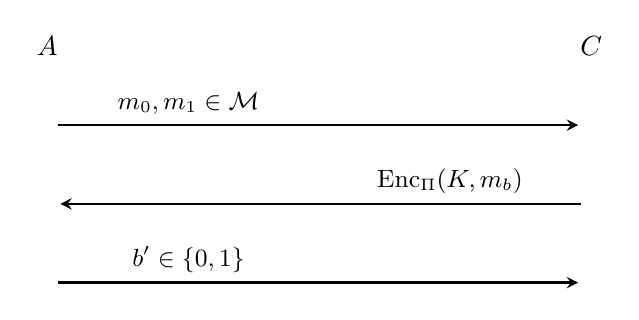
\begin{tikzpicture}[->,>=stealth,shorten >=1pt,auto,node distance=1cm,thick,main node/.style={scale=0.8,circle,draw,font=\sffamily\normalsize}]
            \node[] (1) []{$A$};
            \node[] (2) [left of = 1, xshift = 225]{$C$};

            \node[] (3) [below of = 1]{};
            \node[] (4) [below of = 2]{};

            \node[] (5) [below of = 3]{};
            \node[] (6) [below of = 4]{};

            \node[] (7) [below of = 5]{};
            \node[] (8) [below of = 6]{};

            \path[every node/.style={font=\sffamily\small}]
                (3) edge[near start] node{$m_0, m_1 \in \mathcal{M}$} (4)
                (6) edge[swap, near start] node{$\mathrm{Enc}_\Pi(K, m_b)$} (5)
                (7) edge[near start] node{$b' \in \{0,1\}$} (8)
                ;
        \end{tikzpicture}

        \caption{Graphical representation of $\mathrm{Game}_{\Pi, A}^{\text{1-time}}(\lambda, b)$}
    \end{figure}

    By the very definition of the game, it's easy to see that if, for every pair of messages, the adversary is not capable of distinguishing which message got encrypted by the challenger, i.e. if they are playing $\mathrm{Game}_{\Pi, A}^{\text{1-time}}(\lambda, 0)$ or $\mathrm{Game}_{\Pi, A}^{\text{1-time}}(\lambda, 1)$, then the scheme can be considered \textbf{1-time computationally secure SKE}.

    \begin{frameddefn}{1-time computational security}
        Let $\Pi = (\mathrm{Enc}, \mathrm{Dec})$ be a SKE. We say that $\Pi$ is 1-time computationally secure if:
        \[\mathrm{Game}_{\Pi, A}^{\text{1-time}}(\lambda, 0) \approx_c \mathrm{Game}_{\Pi, A}^{\text{1-time}}(\lambda, 1)\]
    \end{frameddefn}

    To see how this game can be used for specific cryptosystems, we prove that PRG-OTP has 1-time computationally security.

    \begin{framedprop}{}
        PRG-OTP has 1-time computational security.
    \end{framedprop}

    \begin{proof}
        Let $\ell = \poly(n)$ be the expansion factor of the PRG $G$ used inside PRG-OTP. We use an argument similar to the hybrid argument. Let $\mathrm{Hyb}(\lambda, b)$ be the 2-player game defined as follows:
        \begin{enumerate}
            \item The adversary $A$ sends two messages $m_0, m_1 \in \{0,1\}^\lambda$ to the challenger $C$
            \item $C$ picks $z \in_R U_{\lambda+\ell}$ and sends $z \oplus m_b = c$ back to $A$
            \item $A$ analyzes $c$ and tries to guess if it was obtained through $m_0$ or $m_1$ by sending a bit $b' \in \{0,1\}$
            \item If $b' \neq b$, the challenger wins. Otherwise, the adversary wins. 
        \end{enumerate}

        We observe that the difference between $\mathrm{Game}_{\Pi, A}^{\text{1-time}}(\lambda, b)$ and $\mathrm{Hyb}(\lambda, b)$ is given by $G(K)$ being replaced by a uniform at random string $z \in_R U_{\lambda+\ell}$. Since $G(U_\lambda) \approx_c U_{\lambda+\ell}$ by choice of $G$, the hybrid game and the original game are expected to also be indistinguishable from each other.
        
        \textbf{Claim}: For each $b \in \{0,1\}$ it holds that $\mathrm{Game}_{\Pi, A}^{\text{1-time}}(\lambda, b) \approx_c \mathrm{Hyb}(\lambda, b)$

        \begin{proof}[Proof of the claim.]
            By way of contradiction, assume that there is an adversary $A$ such that:
            \[\abs{\Pr\sbk{A(b') = 1 : b' \gets \mathrm{Game}_{\Pi, A}^{\text{1-time}}(\lambda, b)} - \Pr\sbk{A(b') = 1 : b' \gets \mathrm{Hyb}(\lambda, b)}} \geq \frac{1}{\lambda^c}\]

            for some $c > 0$. We build an adversary $D$ defined as follows:

            $D$ = "On input $z \in \{0,1\}^{\lambda+\ell}$.
            \begin{enumerate}
                \item $D$ challenges $A$ to play $\mathrm{Hyb}(\lambda, b)$ (thus $D$ is the challenger and $A$ is the adversary). $D$ will use $z$ to compute $m_b \oplus z = c$ instead of choosing a random string.
                \item $D$ accepts if $A$ wins, otherwise $D$ rejects."
            \end{enumerate}

            Since $A$ can distinguish the two games, it is also able to distinguish if the string $c$ passed by $D$ was computed with $z$ taken from $G(U_\lambda)$ or $U_{\lambda+\ell}$. This implies that:
            \[\Pr[D(z) = 1 : z \in_R G(U_\lambda)] = \Pr\sbk{A(b') = 1 : b' \gets \mathrm{Game}_{\Pi, A}^{\text{1-time}}(\lambda, b)}\]

            and:
            \[\Pr[D(z) = 1 : z \in_R U_{\lambda+\ell}] = \Pr\sbk{A(b') = 1 : b' \gets \mathrm{Hyb}(\lambda, b)}\]

            concluding that:
            \[\begin{split}
                &\abs{\Pr[D(z) = 1 : z \in_R G(U_\lambda)] - \Pr[D(z) = 1 : z \in_R U_{\lambda+\ell}]} \\
                =& \abs{\Pr\sbk{A(b') = 1 : b' \gets \mathrm{Game}_{\Pi, A}^{\text{1-time}}(\lambda, b)} - \Pr\sbk{A(b') = 1 : b' \gets \mathrm{Hyb}(\lambda, b)}} \\
                \geq& \frac{1}{\lambda^c}
            \end{split}\]

            and thus contradicting the fact that $G$ is a PRG.
        \end{proof}
        
        By definition, it's easy to see that $\mathrm{Hyb}(\lambda, 0) \equiv \mathrm{Hyb}(\lambda, 1)$ since the distribution of $c$ is uniform and independent of $b$. Therefore, we conclude that:
        \[\mathrm{Game}_{\Pi, A}^{\text{1-time}}(\lambda, 0) \approx_c \mathrm{Hyb}(\lambda, 0) \equiv \mathrm{Hyb}(\lambda, 1) \approx_c \mathrm{Game}_{\Pi, A}^{\text{1-time}}(\lambda, 1)\]
    \end{proof}

    \section{CPA security and pseudorandom functions}

    In the previous section we proved that PRG-OTP is 1-time computationally secure, meaning that it is secure against attackers that know only one message. However, this SKE's weakness is \textit{cyphertext attacks}. Suppose that an attacker knows a cyphertext-message pair $(m_1, c_1)$. If the challenger sends another cyphertext $c_2$ obtained from a message $m_2$, the attacker is able to retrieve the contents of $m_2$ through the SKE itself:
    \[c_1 \oplus c_2 \oplus m_1 = (G(K) \oplus m_1) \oplus (G(K) \oplus m_2) \oplus m_1 = m_2\]
    
    The generalization of this type of attack is known as \textbf{Known-plaintext Attack (KPA)} and the security counterpart is known as \textit{$t$-time computational security}. We observe that KPAs require that the attacker only knows the pairs $(m_1, c_1), \ldots, (m_t, c_t)$ but is not able to choose them. When the attacker is able to choose the pairs (e.g. they can choose messages and get their cyphertexts) we talk about \textbf{Chosen-plaintext Attack (CPA)}.
    
    In the CPA game the adversary is given access to an encryption \textbf{oracle}, i.e. a sub-procedures with unlimited power that can be queried in order to get an answer. Each query costs $\Theta(1)$ computational steps. We observe that the oracle queries made by the attacker can be seen as \curlyquotes{questions already answered}. For instance, suppose that the attacker queries an oracle $O$ capable of returning the cyphertext of a message, i.e. solves the problem $\mathrm{Enc}(K, \cdot)$. If the attacker queries $m_1, \ldots, m_t$, the oracle will answer with $c_1, \ldots, c_t$. This is equivalent to saying that the attacker has chosen the pairs $(m_1, c_1), \ldots, (m_t, c_t)$. The concept of oracle is just a computational medium to express this idea.
    
    Let $\mathrm{Game}_{\Pi,A}^{\text{CPA}}(\lambda,b)$ be the 2-player game defined as follows:
    \begin{enumerate}
        \item The challenger $C$ generates a key $K \in \mathcal{K}$.
        \item The adversary $A$ queries $m_1, \ldots, m_t \in \{0,1\}^\lambda$, where $t = \poly(\lambda)$, to an oracle for $\mathrm{Enc}_{\Pi}(K, \cdot)$. The oracle answers with $c_1, \ldots, c_t$.
        \item The adversary sends to messages $m_0^*, m_1^* \in \{0,1\}^\lambda$ to the challenger $C$
        \item $C$ sends $\mathrm{Enc}_\Pi(K, m^*_b) = c^*$ back to $A$
        \item $A$ analyzes $c$ and tries to guess if it was obtained through $m_0$ or $m_1$ by sending a bit $b' \in \{0,1\}$
        \item If $b' \neq b$, the challenger wins. Otherwise, the adversary wins. 
    \end{enumerate}

    \begin{figure}[H]
        \centering

        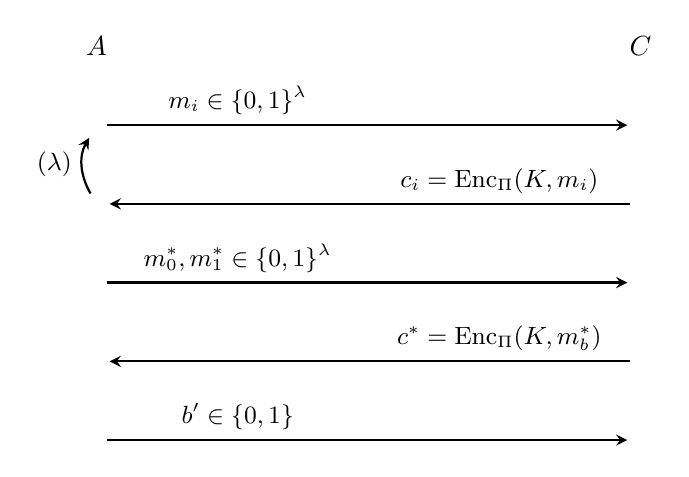
\begin{tikzpicture}[->,>=stealth,shorten >=1pt,auto,node distance=1cm,thick,main node/.style={scale=0.8,circle,draw,font=\sffamily\normalsize}]
            \node[] (1) []{$A$};
            \node[] (2) [left of = 1, xshift = 225]{$C$};

            \node[] (3) [below of = 1]{};
            \node[] (4) [below of = 2]{};

            \node[] (5) [below of = 3]{};
            \node[] (6) [below of = 4]{};

            \node[] (7) [below of = 5]{};
            \node[] (8) [below of = 6]{};

            \node[] (9) [below of = 7]{};
            \node[] (10) [below of = 8]{};

            \node[] (11) [below of = 9]{};
            \node[] (12) [below of = 10]{};

            \path[every node/.style={font=\sffamily\small}]
                (5) edge[bend left] node {$\poly(\lambda)$}(3)
                (3) edge[near start] node{$m_i \in \{0,1\}^\lambda$} (4)
                (6) edge[swap, near start] node{$c_i = \mathrm{Enc}_\Pi(K, m_i)$} (5)
                (7) edge[near start] node{$m_0^*, m_1^* \in \{0,1\}^\lambda$} (8)
                (10) edge[swap, near start] node{$c^* = \mathrm{Enc}_\Pi(K, m_b^*)$} (9)
                (11) edge[near start] node{$b' \in \{0,1\}$} (12)
                ;
        \end{tikzpicture}

        \caption{Graphical representation of $\mathrm{Game}_{\Pi, A}^{\text{CPA}}(\lambda, b)$. Queries to the oracle can be substituted with queries to $C$, as if the two players already exchanged some pairs.}
    \end{figure}

    \begin{frameddefn}{CPA-security}
        Let $\Pi = (\mathrm{Enc}, \mathrm{Dec})$ be a SKE. We say that $\Pi$ is CPA-secure if:
        \[\mathrm{Game}_{\Pi, A}^{\text{CPA}}(\lambda, 0) \approx_c \mathrm{Game}_{\Pi, A}^{\text{CPA}}(\lambda, 1)\]
    \end{frameddefn}

    It's easy to see that the PRG-OTP is not CPA-secure since the output of the encryption scheme is \textit{deterministic} (meaning that it will always return the same output when given the same input). Consider the attacker that queries two messages $m_0, m_1 \in \{0,1\}^n$. After obtaining the cyphertexts $c_0, c_1$ from $C$, the attacker sends the final queries $m_0^* = m_0$ and $m_1^* = m_1$, obtaining the final cyphertext $c^*$. Since the scheme is deterministic, we know that either $c^* = c_0$ or $c^* = c_1$ must hold (depending on the value $b$ used by $C$). Thus, the attacker returns 0 if $c^* = c_0$,, otherwise they returns 1. This allows the attacker to distinguish the two games with probability 1. We observe that this idea is not restricted to the PRG-OTP: it holds for any deterministic SKE!

    \begin{framedprop}{}
        No deterministic SKE can be CPA-secure.
    \end{framedprop}

    In order to make a CPA-secure SKE, we need to substitute pseudorandom generators with \textbf{pseudorandom functions}, i.e. functions that are indistinguishable from a randomly selected one (thus they make their internal workings incomprehensible).

    Let $\mathcal{R}(s \to t)$ denote the uniform distribution over the set of all functions from strings of $s$ bits to strings of $t$ bits. We define the following 2-player game $\mathrm{Game}_{\mathcal{F},A}^{\text{PRF}}(\lambda, b)$:
    \begin{enumerate}
        \item The challenger $C$ generates a key $K \in \{0,1\}^\lambda$ and sets $H = F_K$ if $b = 0$, otherwise $H \in_R \mathcal{R}(n \to n)$.
        \item The adversary $A$ queries $x_1, \ldots, x_t \in \{0,1\}^n$ where $t = \poly(n)$, to an oracle for $H(\cdot)$. The oracle answers with $y_1, \ldots, y_t$.
        \item $A$ tries to guess $b$ by sending a bit $b' \in \{0,1\}$
        \item If $b \neq b'$, the challenger wins. Otherwise, the adversary wins.
    \end{enumerate}

    \begin{figure}[H]
        \centering

        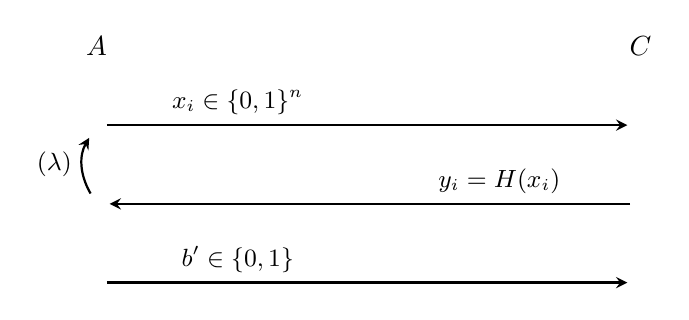
\begin{tikzpicture}[->,>=stealth,shorten >=1pt,auto,node distance=1cm,thick,main node/.style={scale=0.8,circle,draw,font=\sffamily\normalsize}]
            \node[] (1) []{$A$};
            \node[] (2) [left of = 1, xshift = 225]{$C$};

            \node[] (3) [below of = 1]{};
            \node[] (4) [below of = 2]{};

            \node[] (5) [below of = 3]{};
            \node[] (6) [below of = 4]{};


            \node[] (11) [below of = 5]{};
            \node[] (12) [below of = 6]{};

            \path[every node/.style={font=\sffamily\small}]
                (5) edge[bend left] node {$\poly(\lambda)$}(3)
                (3) edge[near start] node{$x_i \in \{0,1\}^n$} (4)
                (6) edge[swap, near start] node{$y_i = H(x_i)$} (5)
                (11) edge[near start] node{$b' \in \{0,1\}$} (12)
                ;
        \end{tikzpicture}

        \caption{Graphical representation of $\mathrm{Game}_{\mathcal{F}, A}^{\text{PRF}}(\lambda, b)$. Queries to the oracle can be substituted with queries to $C$, as if the two players already exchanged some pairs.}
    \end{figure}

    \begin{frameddefn}{Pseudorandom functions}
        Let $\mathcal{F} = \{F_K : \{0,1\}^n \to \{0,1\}^m\}_{K \in \{0,1\}^\lambda}$ be a family of poly-time functions. We say that $\mathcal{F}$ is a pseudorandom function family (PRF) if:
        \[\mathrm{Game}_{\mathcal{F},A}^{\text{PRF}}(\lambda, 0) \approx_c \mathrm{Game}_{\mathcal{F},A}^{\text{PRF}}(\lambda, 1)\]
    \end{frameddefn}

    We observe that the above definition requires that $\mathcal{F}$ is a family of efficient \underline{deterministic} functions: randomness is only used to choose a key that identifies which function of the family must be used. The uniform distribution $\mathcal{R}(n \to n)$, instead, also contains functions that aren't poly-time computable. The idea behind the PRF game is to establish that each function of the family is computationally indistinguishable from a randomly chosen function.

    In practical applications, many common encryption schemes (e.g. DES, 3DES, AES, \dots) are based on on \textit{pseudorandom permutations (PRP)}, i.e. PRFs that are invertible if they key is known. For now, we'll give the idea behind how PRFs can be used in theory to produce CPA-secure SKEs.
    
    First of all, we observe that we cannot simply swap PRGs with PRFs in order to get a good scheme since each function is deterministic. The trick here is to use a random initial value called \textbf{nonce} (short for \curlyquotes{number used once}). As their name suggests, these values are used exactly once by the cryptosystem, granting that the same input will always give a different cyphertext.
    
    Given a PRF $\mathcal{F} = \{F_K : \{0,1\}^n \to \{0,1\}^n\}_{K \in \{0,1\}^\lambda}$, let the \textit{PRF One Time Pad (PRF-OTP)} be the scheme defined by the following operations:
    \begin{enumerate}
        \item $\mathrm{Enc}(K,m) = (r, F_K(r) \oplus m)$, where $r \in \{0,1\}^n$ is a nonce
        \item $\mathrm{Dec}(K,(r,c)) = F_K(r) \oplus c$
    \end{enumerate}
    
    We observe that the encryption operation must also return the used nonce in order for the decryption operation to work. However, this is not an issue for CPA-security: since the nonce will never be used again by the scheme, the adversary gains no information on the key by knowing it.

    \begin{framedprop}{}
        PRF-OTP is CPA-secure.
    \end{framedprop}

    \begin{proof}
        Omitted (an hybrid argument suffices).
    \end{proof}

    \subsection{The GGM Tree}
    
    After discussing how PRFs can be used to achieve CPA-security, we prove that PRGs can be used to construct PRFs. In particular, we'll give an explicit construction known as the \textbf{Goldreich-Goldwasser-Micali Tree (GGM Tree)}.

    \begin{frameddefn}{GGM Tree}
        Given a PRG $G : \{0,1\}^\lambda \to \{0,1\}^{2\lambda}$, let $G_0, G_1 : \{0,1\}^\lambda \to \{0,1\}^\lambda$ be two functions that respectively return the first and last $\lambda$ bits of the output of $G$, meaning that $G(k) = G_0(k) \concat G_1(k)$ for all $k \in \{0,1\}^\lambda$. The GGM Tree function family is defined as $\mathcal{F} = \{F_K : \{0,1\}^n \to \{0,1\}^\lambda\}_{K \in \{0,1\}^\lambda}$, where:
        \[F_K(x_1 \concat \ldots \concat x_n) = G_{x_n}(G_{x_{n-1}}(\ldots G_{x_2}(G_{x_1}(K))))\]
    \end{frameddefn}


    \begin{figure}[H]
        \centering

        \begin{tikzpicture}[
            edge from parent/.style={draw, -{Latex[length=2mm]}, thick},
            every node/.style={font=\small},
            level distance=1.8cm,
            level 1/.style={sibling distance=8cm},
            level 2/.style={sibling distance=4cm},
            level 3/.style={sibling distance=2cm}
        ]
            \node {$K$}
                child {node {$G_0(K)$}
                    child {node {$G_0(G_0(K))$}
                    child {node[rectangle, draw] {$F_K(000)$} edge from parent node[left] {0}}
                    child {node[rectangle, draw] {$F_K(001)$} edge from parent node[right] {1}}
                    edge from parent node[left, yshift=5] {0}
                    }
                    child {node {$G_1(G_0(K))$}
                    child {node[rectangle, draw] {$F_K(010)$} edge from parent node[left] {0}}
                    child {node[rectangle, draw, color=Red] {$F_K(011)$} edge from parent node[right] {1}}
                    edge from parent node[right, yshift=5] {1}
                    }
                    edge from parent node[left, yshift=5] {0}
                }
                child {node {$G_1(K)$}
                    child {node {$G_0(G_1(K))$}
                    child {node[rectangle, draw] {$F_K(100)$} edge from parent node[left] {0}}
                    child {node[rectangle, draw] {$F_K(101)$} edge from parent node[right] {1}}
                    edge from parent node[left, yshift=5] {0}
                    }
                    child {node {$G_1(G_1(K))$}
                    child {node[rectangle, draw] {$F_K(110)$} edge from parent node[left] {0}}
                    child {node[rectangle, draw] {$F_K(111)$} edge from parent node[right] {1}}
                    edge from parent node[right, yshift=5] {1}
                    }
                    edge from parent node[right, yshift=5] {1}
                };
        \end{tikzpicture}

        \caption{The GGM Tree for inputs of length $n = 3$. The path leading to the red rectangle represent the computation $F_K(011) = G_1(G_1(G_0(K)))$.}
    \end{figure}
    
    \begin{framedlem}[label={t_prg_uniform}]{}
        Let $G : \{0,1\}^\lambda \to \{0,1\}^{2\lambda}$ be a PRG. Given $K_1, \ldots, K_t \in_R U_\lambda$, with $t = \poly(\lambda)$ and $K_i \neq K_j$ for all $i \neq j$, it holds that:
        \[(G(K_1), \ldots, G(K_t)) \approx_c (U_{2\lambda}, \ldots, U_{2\lambda})\] 
    \end{framedlem}

    \begin{proof}
        We define $t$ hybrid distributions $H_0, \ldots, H_t$ such that for each $i \in [t]$ it holds that:
        \[H_i = (G(K_1), \ldots, G(K_{t-i}), \underbrace{U_{2\lambda}, \ldots, U_{2\lambda}}_{i \text{ times}})\]

        We observe that $H_0 \equiv (G(K_1), \ldots, G(K_t))$ and $H_t \equiv (U_{2\lambda}, \ldots, U_{2\lambda})$.

        \textbf{Claim:} For each $i \in [0,t-1]$ it holds that $H_i \approx_c H_{i+1}$.

        \begin{proof}[Proof of the claim]
            Fix $i \in [0, t-1]$. We prove the claim by reducing the distinguishability of $G(K_{t-i})$ from $U_{2\lambda}$ to the distinguishability of $H_i$ from $H_{i+1}$. By way of contradiction, suppose that $H_i \not\approx_c H_{i+1}$, meaning that there is a distinguisher $D_i$ such that:
            \[\abs{\Pr[D_i(z) = 1 : z \in_R H_i] - \Pr[D_i(z) = 1 : z \in_R H_{i+1}]} > \frac{1}{n^c}\]
            for some $c > 0$. Let $D$ be the algorithm defined as follows:

            $D$ = "On input $z \in \{0,1\}^{2\lambda}$:

            \begin{enumerate}
                \item Extract $t-i$ keys $K_1, \ldots, K_{t-i} \in_R U_\lambda$
                \item Extract $i-1$ strings $w_{1}, \ldots, w_{i-1} \in_R U_{2\lambda}$
                \item Return $D_i(G(K_1) \concat \ldots \concat G(K_{t-i}) \concat z \concat w_1 \concat \ldots \concat w_{i-1})$"
            \end{enumerate}
            
            We observe that $H_i$ and $H_{i+1}$ differ only on the $i$-th string of $2n$ bits: the former contains an output of $G$ while the latter contains a truly random strng. This implies that:
            \[\begin{split}
                &\abs{\Pr[D(w) = 1 : w \in_R G(K_{t-i})] - \Pr[D(w) = 1 : w \in_R U_{2\lambda}]}\\
                = &\abs{\Pr[D_i(z') = 1 : z' \in_R H_i] - \Pr[D_i(z') = 1 : z' \in_R H_{i+1}]} \\
                > &\frac{1}{n^c}
            \end{split}\]
            concluding that $D$ is a distinguisher for $G$, raising a contradiction over $G$ being a PRG.
        \end{proof}
         
        By transitivity of $\approx_c$, the claim concludes that:
        \[(G(K_1), \ldots, G(K_t)) \equiv H_0 \approx_c \ldots \approx_c H_t \equiv (U_{2\lambda}, \ldots, U_{2\lambda})\]
    \end{proof}

    \begin{framedthm}{The GGM theorem}
        GGM Tree is a PRF when constructed using a PRG
    \end{framedthm}

    \begin{proof}
        Let $G : \{0,1\}^\lambda \to \{0,1\}^{2\lambda}$ be a PRG and let $G_0, G_1 : \{0,1\}^\lambda \to \{0,1\}^\lambda$ be the two functions such that $G(x) = G_0(x) \concat G_1(x)$. Let also $\mathcal{F} = \{F_K : \{0,1\}^n \to \{0,1\}^\lambda\}_{K \in \{0,1\}^\lambda}$ be the GGM function family.

        Fix a key $K \in \{0,1\}^\lambda$. We proceed by induction on the length $n$ of the input. When $n = 1$ it holds that $F_K(x) = G_x(K)$. Since $U_{2\lambda} \approx_c G(K) \equiv (G_0(K), G_1(K))$, we know that $G_0(K) \approx_c U_\lambda$ and $G_1(K) \approx_c U_\lambda$. This concludes that, independently from the value of $x$, the output $F_K(x)$ is undistinguishable from a string taken from $U_\lambda$, making it undistinguishable from a random function taken from $\mathcal{R}(1 \to \lambda)$. 

        We now assume that the inductive hypothesis holds for $n-1$, i.e. that the GGM family $\mathcal{F} = \{F_K : \{0,1\}^{n-1} \to \{0,1\}^{\lambda}\}_{K \in \{0,1\}^\lambda}$ is a PRF. First, we observe that for each key $K \in \{0,1\}^\lambda$, for each $x \in \{0,1\}^n$ and for each $y \in \{0,1\}^{n-1}$ it holds that $F_K(x \concat y) = G_{x}(F_K'(y))$.
        
        We define the following three hybrid distributions:
        \begin{itemize}
            \item $\mathrm{Hyb}_0$ is the distribution over the function $F_K(x \concat y) = G_x(F_K'(y))$
            \item $\mathrm{Hyb}_1$ is the distribution over the function $H(x \concat y) = G_x(R'(y))$ where $R' \in_R \mathcal{R}(n-1 \to \lambda)$.
            \item $\mathrm{Hyb}_2$ is the distribution over the function $R \in_R \mathcal{R}(n \to \lambda)$.
        \end{itemize}

        To prove that $\mathcal{F}$ is also a PRF, we'll show that $\mathrm{Hyb}_0 \approx_c \mathrm{Hyb}_1 \approx_c \mathrm{Hyb}_2$.
        
        \textbf{Claim 1}: $\mathrm{Hyb}_0 \approx_c \mathrm{Hyb}_1$
        
        \begin{proof}[Proof of Claim 1]
            We reduce the distinguishability of $\mathrm{Game}_{\mathcal{F}',A}^{\text{PRF}}(\lambda, 0)$ from $\mathrm{Game}_{\mathcal{F}',A}^{\text{PRF}}(\lambda, 1)$ to the distinguishability of $\mathrm{Hyb}_0$ from $\mathrm{Hyb}_1$. By way of contradiction, suppose that $\mathrm{Hyb}_0 \not\approx_c \mathrm{Hyb}_{1}$, meaning that there is a PPT adversary $D_{01}$ such that:
            \[\abs{\Pr[D_{01}(z) = 1 : z \in_R \mathrm{Hyb}_0] - \Pr[D_{01}(z) = 1 : z \in_R \mathrm{Hyb}_1]} > \frac{1}{n^c}\]
            for some $c > 0$. We define the attack strategy $A_{01}$ for $\mathrm{Game}_{\mathcal{F}',A}^{\text{PRF}}(\lambda, b)$ as follows. The idea is for $A_{01}$ to play two games simultaneously.

            \begin{enumerate}
                \item The challenger $C$ generates a key $K \in \{0,1\}^\lambda$ and sets $H = F'_K$ if $b = 0$, otherwise $H \in_R \mathcal{R}(n-1 \to \lambda)$.
                \item $A_{01}$ challenges $D_{01}$ to distinguish $\mathrm{Hyb}_0$ from $\mathrm{Hyb}_1$.
                \item For each query $x \concat y$ -- with $x \in \{0,1\}$ and $y \in \{0,1\}^n$ -- made by $D_{01}$, the adversary $A_{01}$ forwards $y$ to the challenger $C$.
                \item For each answer $z$ returned by $C$, the adversary $A_{01}$ forwards $G_x(z)$ to $D_{01}$.
                \item When $D_{01}$ gives the final bit $b'$, $A_{01}$ forwards the same bit to $C$.
            \end{enumerate}

            In the above strategy, $A_{01}$ plays two games simultaneously, using the challenger as a way to compute outputs of either $F'_K$ or a random function $R$. After obtaining the outputs, $A_{01}$ passes them through $G_x$ before forwarding them to $D_{01}$. If the challenger used $F'_K$, the values forwarded from $A_{01}$ will be outputs of $F_K$. Otherwise, if the challenger used $R'$, the values forwarded from $A_{01}$ will be outputs of $R$. Since $D_{01}$ can distinguish between $F_K$ and $R$, $A_{01}$ will be able to distinguish $F'_K$ from $R'$. This contradicts the fact that $\mathcal{F}'$ is a PRF, concluding that $\mathrm{Hyb}_0 \approx_c \mathrm{Hyb}_{1}$ must be true.
        \end{proof}

        \textbf{Claim 2}: $\mathrm{Hyb}_1 \approx \mathrm{Hyb}_2$

        \begin{proof}[Proof of Claim 2]
            We reduce the distinguishability of $(G(K_1), \ldots, G(K_t))$ from $(U_{2\lambda}, \ldots, U_{2\lambda})$ to the distinguishability of $\mathrm{Hyb}_1$ from $\mathrm{Hyb}_2$. By way of contradiction, suppose that there is an algorithm $D_{12}$ that distinguishes $\mathrm{Hyb}_1$ from $\mathrm{Hyb}_{2}$
            For each string $w \in \{0,1\}^{2\lambda}$, let $w^0, w^1 \in \{0,1\}^{\lambda}$ denote the first and last $\lambda$ bits of $w$, i.e. $w = w^0 \concat w^1$. Let $A_{12}$ be the algorithm defined as follows:

            $A_{12}$ = "On input $z = z_1 \concat \ldots \concat z_t$ with $z_i \in \{0,1\}^{2\lambda}$:

            \begin{enumerate}
                \item $A_{12}$ challenges $D_{12}$ to distinguish $\mathrm{Hyb}_1$ from $\mathrm{Hyb}_2$, allowing $D_{12}$ exactly $t$ queries.
                \item For each query $x \concat y$ -- with $x \in \{0,1\}$ and $y \in \{0,1\}^n$ -- made by $D_{12}$, the adversary $A_{12}$ answers with $z^x_{i(y)}$, where $i(y) \in [1,t]$ is either the index that was used by $A_{12}$ if $D_{12}$ already queried $y$ or the next unused index.
                \item When $D_{01}$ gives the final bit $b'$, $A_{01}$ returns $b'$
            \end{enumerate}

            When $z_1, \ldots, z_t \in U_{2\lambda}$, all values returned by $A_{12}$ to $D_{12}$ will be truly random, making $D_{12}$ assume that the values are taken from the distribution $\mathrm{Hyb}_2$. When $z_1, \ldots, z_t \in G(U_{\lambda})$, instead, all values will be outputs of $G$, making $D_{12}$ assume that the values are taken from the distribution $\mathrm{Hyb}_1$. This concludes that $A_{12}$ is a distinguisher for $(G(K_1), \ldots, G(K_t))$ and $(U_{2\lambda}, \ldots, U_{2\lambda})$, contradicting \Cref{t_prg_uniform}.
        \end{proof}
    \end{proof}

    \begin{figure}[H]
        \centering

        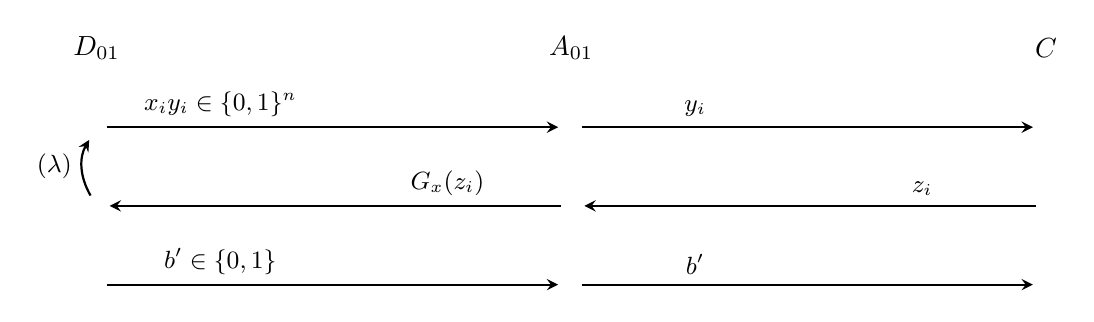
\begin{tikzpicture}[->,>=stealth,shorten >=1pt,auto,node distance=1cm,thick,main node/.style={scale=0.8,circle,draw,font=\sffamily\normalsize}]
            \node[] (1) []{$D_{01}$};
            \node[] (2) [left of = 1, xshift = 200]{$A_{01}$};
            \node[] (2x) [left of = 2, xshift = 200]{$C$};

            \node[] (3) [below of = 1]{};
            \node[] (4) [below of = 2]{};
            \node[] (4x) [below of = 2x]{};

            \node[] (5) [below of = 3]{};
            \node[] (6) [below of = 4]{};
            \node[] (6x) [below of = 4x]{};


            \node[] (11) [below of = 5]{};
            \node[] (12) [below of = 6]{};
            \node[] (12x) [below of = 6x]{};

            \path[every node/.style={font=\sffamily\small}]
                (5) edge[bend left] node {$\poly(\lambda)$}(3)
                
                (3) edge[near start] node{$x_i \concat y_i \in \{0,1\}^{n}$} (4)
                (6) edge[swap, near start] node{$G_x(z_i)$} (5)
                (11) edge[near start] node{$b' \in \{0,1\}$} (12)

                (4) edge[near start] node{$y_i$} (4x)
                (6x) edge[swap, near start] node{$z_i$} (6)
                (12) edge[near start] node{$b'$} (12x)
                ;
        \end{tikzpicture}

        \caption{Graphical representation of the double-game attack used to prove Claim 1 of the GGM theorem.}
    \end{figure}


    \begin{figure}[H]
        \centering

        \begin{tikzpicture}[->,>=stealth,shorten >=1pt,auto,node distance=1cm,thick,main node/.style={scale=0.8,circle,draw,font=\sffamily\normalsize}]
            \node[] (1) []{$D_{12}$};
            \node[] (2) [left of = 1, xshift = 200]{$A_{12}$};
            \node[] (2x) [left of = 2, xshift = 200]{$C$};
            
            \node[] (a) [below of = 1]{};
            \node[] (b) [below of = 2]{};
            \node[] (c) [below of = 2x]{};

            \node[] (3) [below of = a]{};
            \node[] (4) [below of = b]{};
            \node[] (4x) [below of = c]{};

            \node[] (5) [below of = 3]{};
            \node[] (6) [below of = 4]{};
            \node[] (6x) [below of = 4x]{};


            \node[] (11) [below of = 5]{};
            \node[] (12) [below of = 6]{};
            \node[] (12x) [below of = 6x]{};

            \path[every node/.style={font=\sffamily\small}]
                (5) edge[bend left] node {$t$}(3)

                (c) edge[swap, near start] node{$z_i \concat \ldots \concat z_t \in \{0,1\}^{2\lambda t}$} (b)
                
                (3) edge[near start] node{$x_j \concat y_j \in \{0,1\}^{n}$} (4)
                (6) edge[swap, near start] node{$z^{x_j}_{i(y_j)}$} (5)
                (11) edge[near start] node{$b' \in \{0,1\}$} (12)

                (12) edge[near start] node{$b'$} (12x)
                ;
        \end{tikzpicture}

        \caption{Graphical representation of the double-game attack used to prove Claim 2 of the GGM theorem.}
    \end{figure}

    \section{Encryption modes for SKEs}

    After proving that OWFs can be used to create PRFs through PRGs, we're going to show that PRFs are enough to achieve practical symmetric-key encryption. As we'll see, for some practical applications we strictly require that the pseudorandom functions are invertible, i.e. that they are PRPs. Practical functions with this property are commonly called \textbf{blockchiphers} (the concept of blockchipers was used way before the introduction of the concept of PRPs). From a theoretical prospective, we'll discuss how PRFs can be used to derive PRPs. From a practical prospective, instead, we'll discuss some blockchipers used in the real world.

    First of all, we observe that real-world encryption systems must work with messages of \textit{different lengths}. Formally, we say that these SKEs have \textbf{Variable Input Length (VIL)}, meaning that for each message $m$ it holds that $\abs{m} = \poly(\lambda)$, where $\lambda$ is the key length. In order to achieve security for VIL SKEs, we require a \curlyquotes{standardized way} to encrypt messages of variable length. To solve this issue, each message $m$ is split into a variable number of \textbf{blocks} of an equal fixed length $n$ (commonly is a power of 2, such as 256). In other words, each message $m$ is considered as $m = (m_1, \ldots, m_d)$ where $d \in \N$ and $m_i \in \{0,1\}^n$.
    
    The simplest encryption type is the \textbf{Electronic Code Book (ECB)} mode, where the scheme simply applies the selected PRF to every block of the message.
    
    \begin{frameddefn}{Electronic Code Book (ECB) mode}
        Let $\mathcal{F} = \{F_K : \{0,1\}^n \to \{0,1\}^n\}_{K \in \{0,1\}^\lambda}$ be a PRF. Let $K \in \{0,1\}^\lambda$ be a chosen key. On input $m = (m_1, \ldots, m_d)$ the ECB encryption mode returns the cyphertext $c = (c_1, \ldots, c_d)$ constructed as:
        \begin{itemize}
            \item For all $i \in [d]$ it holds that $c_i = F_K(m_i)$
        \end{itemize}
    \end{frameddefn}

    \begin{figure}[H]
        \centering
        \includegraphics[scale=1]{images/ECB.pdf}
        \caption{Graphical representation of ECB mode.}
    \end{figure}
    
    Clearly, the ECB mode cannot be CPA-secure since it is deterministic. As discussed in the PRF-OTP example, a nonce value is sufficient to make the ecryption non-deterministic. In encryption modes, this nonce value is usually referred to as \textbf{Initialization Vector (IV)}. In order to make decryption harder to bruteforce, common encryption modes are based on \textit{sequential encryption}: some value produced during the encryption of block $m_i$ is used for the encryption of block $m_{i+1}$. This allows us to restrict our interests to the secretness of the key and the IV. Moreover, it also makes decryption unparallelizable, further improving the security of the SKE. The first type of encryption mode based on this idea is the \textbf{Cipher Block Chaining (CBC)}.

    \begin{frameddefn}{Cipher Block Chaining (CBC) mode}
        Let $\mathcal{F} = \{F_K : \{0,1\}^n \to \{0,1\}^n\}_{K \in \{0,1\}^\lambda}$ be a PRF. Let $K \in \{0,1\}^\lambda$ be a chosen key. On input $m = (m_1, \ldots, m_d)$ the CBC encryption mode returns the cyphertext $c = (c_1, \ldots, c_d)$ constructed as:
        \begin{itemize}
            \item $c_0 \in_R U_n$ is a nonce value (IV)
            \item For all $i \in [d]$ it holds that $c_i = F_K(c_{i-1} \oplus m_i)$
        \end{itemize}
    \end{frameddefn}

    \begin{figure}[H]
        \centering
        \includegraphics[scale=1]{images/CBC.pdf}
        \caption{Graphical representation of CBC mode.}
    \end{figure}

    Other types of encryption mode are pretty much based on ideas similar to CBC. The only real difference lies in the order of operations. For instance, the \textbf{Cipher Feedback (CFB)} mode XORes each block after applying the PRF to the nonce value, instead of before. We observe that this was the idea behind our PRF-OTP example, the only difference lies in the chaining of encryptions.


    \begin{frameddefn}{Cipher Feedback (CFB) mode}
        Let $\mathcal{F} = \{F_K : \{0,1\}^n \to \{0,1\}^n\}_{K \in \{0,1\}^\lambda}$ be a PRF. Let $K \in \{0,1\}^\lambda$ be a chosen key. On input $m = (m_1, \ldots, m_d)$ the CFB encryption mode returns the cyphertext $c = (c_1, \ldots, c_d)$ constructed as:
        \begin{itemize}
            \item $c_0 \in_R U_n$ is a nonce value (IV)
            \item For all $i \in [d]$ it holds that $c_i = F_K(c_{i-1}) \oplus m_i$
        \end{itemize}
    \end{frameddefn}

    \begin{figure}[H]
        \centering
        \includegraphics[scale=1]{images/CFB.pdf}
        \caption{Graphical representation of CFB mode.}
    \end{figure}

    Another encryption mode extremely similar to CFB is the \textbf{Output Feedback (OFB)} mode, where the output of the PRF is directly forwarded instead of being XORed first.

    \begin{frameddefn}{Output Feedback (OFB) mode}
        Let $\mathcal{F} = \{F_K : \{0,1\}^n \to \{0,1\}^n\}_{K \in \{0,1\}^\lambda}$ be a PRF. Let $K \in \{0,1\}^\lambda$ be a chosen key. On input $m = (m_1, \ldots, m_d)$ the OFB encryption mode returns the cyphertext $c = (c_1, \ldots, c_d)$ constructed as:
        \begin{itemize}
            \item $q_0 \in_R U_n$ is a nonce value (IV)
            \item For all $i \in [d]$ it holds that $q_i = F_K(q_{i-1})$
            \item For all $i \in [d]$ it holds that $c_i = q_i \oplus m_i$
        \end{itemize}
    \end{frameddefn}

    \begin{figure}[H]
        \centering
        \includegraphics[scale=1]{images/OFB.pdf}
        \caption{Graphical representation of OFB mode.}
    \end{figure}

    The last standard encryption mode we discuss is \textbf{Counter (CTR)} mode. Instead of using the previous (partial) output as the next input for the PRF, this mode gradually increases the initial nonce value and uses it for the next encryptions.

    \begin{frameddefn}{Counter (CTR) mode}
        Let $\mathcal{F} = \{F_K : \{0,1\}^n \to \{0,1\}^n\}_{K \in \{0,1\}^\lambda}$ be a PRF. Let $K \in \{0,1\}^\lambda$ be a chosen key. On input $m = (m_1, \ldots, m_d)$ the OFB encryption mode returns the cyphertext $c = (c_1, \ldots, c_d)$ constructed as:
        \begin{itemize}
            \item $r \in_R U_n$ is a nonce value (IV)
            \item For all $i \in [d]$ it holds that $c_i = F_K(r+i-1) \oplus m_i$
        \end{itemize}

        \textit{Note}: the sum operation is in mod 2.
    \end{frameddefn}

    \begin{figure}[H]
        \centering
        \includegraphics[scale=1]{images/CTR.pdf}
        \caption{Graphical representation of CTR mode.}
    \end{figure}

    CBC, CFB, OFB and CTR can all be proven to be CPA-secure for VIL. Instead of proving the security of all of them, we'll give an idea by proving the result only for CTR (which is actually harder to prove).
    
    \begin{framedthm}{}
        CBC, CFB, OFB and CTR are CPA-secure for VIL when constructed using a PRF
    \end{framedthm}
\end{document}
